%% LyX 2.0.7 created this file.  For more info, see http://www.lyx.org/.
%% Do not edit unless you really know what you are doing.
\documentclass[a4paper,spanish]{report}
\usepackage[T1]{fontenc}
\usepackage[utf8]{luainputenc}
\usepackage{listings}
\setcounter{secnumdepth}{0}
\setcounter{tocdepth}{3}
\usepackage{array}
\usepackage{pdfpages}
\usepackage{multirow}
\usepackage{amsmath}
\usepackage{amssymb}
\usepackage{graphicx}
\usepackage{esint}

\makeatletter

%%%%%%%%%%%%%%%%%%%%%%%%%%%%%% LyX specific LaTeX commands.
\pdfpageheight\paperheight
\pdfpagewidth\paperwidth

%% Because html converters don't know tabularnewline
\providecommand{\tabularnewline}{\\}
%% A simple dot to overcome graphicx limitations
\newcommand{\lyxdot}{.}


%%%%%%%%%%%%%%%%%%%%%%%%%%%%%% User specified LaTeX commands.
\usepackage{graphicx}
\AtBeginDocument{%
\addto\captionsspanish{%
\renewcommand{\chaptername}{Tema }%
}}
\usepackage{fancyhdr}
\pagestyle{fancy}
\renewcommand{\sectionmark}[1]{\markboth{#1}{}}
\fancyhead[ER,OR,EL,OL]{}
\fancyhead[EC,OC]{\hfill \leftmark}
\cfoot{\thepage} 

\makeatother

\usepackage{babel}
\addto\shorthandsspanish{\spanishdeactivate{~<>}}

\begin{document}
\begin{titlepage}

\includepdf{portada}

\end{titlepage}

\clearpage\thispagestyle{empty}\null\newpage

\tableofcontents{}

\clearpage\thispagestyle{empty}\null\newpage

\pagestyle{fancy}


\chapter{Introducción}


\section{El problema}

Llevar a buen término un proyecto de mecánica orbital es uno de los
procesos más complejos a los que se puede enfrentar un grupo de ingenieros
espaciales. La precisión necesaria en los cálculos, los grandes tiempos
involucrados en el proceso y la inmensa cantidad de datos a generar
hacen que el proyecto resulte largo y tedioso, y requiera numerosas
iteraciones con cálculos y modelos cada vez más refinados. El coste
de todos estos sucesivos pasos es cada vez más elevado, por lo que
resulta de suma importancia asegurarse de que las decisiones tomadas
al principio son adecuadas. 

Los comienzos siempre son duros. Al principio del proyecto se tienen
muy pocos datos y nociones del camino, y los que se tienen están basados
en los juicios y la experiencia de los ingenieros encargados más que
en cálculos específicos. Pero, por desgracia, el problema suele ser
lo suficientemente complejo como para necesitar un apoyo informático
a la hora de realizar los cálculos necesarios para avanzar. Llegado
este punto, se suelen tener tres caminos para elegir como continuar
\begin{itemize}
\item Usar software propio. Si se reutiliza código de proyectos anteriores
es poco probable que esté diseñado para cubrir las variaciones del
actual, y crear un programa diferente para cada proyecto es un proceso
tedioso y que consume mucho tiempo que podría usarse en otra parte.
Esta via proporciona el mayor control sobre el proyecto, pero aumenta
los costes de las críticas primeras etapas.
\item Usar software comercial. Existen numerosas licencias de software creado
por un equipo especializado que cumplen multitud de tareas necesarias
en el proceso. Sin embargo la comercialización de estos paquetes,
normalmente a alto precio, hace que de nuevo los costes de las primeras
etapas suban, siendo inabarcables normalmente para investigadores,
estudiantes o simplemente curiosos. Además, al ser código cerrado,
el ingeniero tiene que fiarse de que cumple los requisitos sin poder
comprobarlo, y no se pueden introducir modificaciones para adecuarlo
y personalizarlo al problema particular.
\item Usar software libre. Hay publicados numerosos programas bajo una licencia
de software libre, que permite acceso al ingeniero al código abierto
del programa. Son altamente personalizables y flexibles, pero se suelen
presentar en forma de librerías de funciones, que a su vez el ingeniero
tiene que unir e implementar para obtener el problema concreto.
\end{itemize}

\section{Objetivos}

En este proyecto se va a intentar, de alguna manera, unificar estas
tres vías en un simulador de órbita baja terrestre, que sea capaz
por si sólo de enfrentarse a las primeras etapas de un proceso de
análisis de misión LEO con cierta precisión, fiabilidad y flexibilidad,
de código abierto que permita a estudiantes e investigadores acceder
y complementar sus funciones sin ningún coste. Para ello se pide que
el programa cumpla los siguientes requisitos:
\begin{itemize}
\item Debe ser sencillo e intuitivo de usar, con una presentación de datos
limpia y clara y una interfaz gráfica amigable que incluya todos los
controles necesarios.
\item Debe abarcar cierto grado de personalización dentro del programa,
permitiendo configurar elementos claves dentro de la simulación. Por
ejemplo, debe dejar elegir qué perturbaciones se quieren utilizar,
o qué datos debe proporcionar.
\item Debe ser personalizable en el código, permitiendo añadir modificaciones
al código base que permitan al ingeniero usar el programa como base
sobre la que construir su problema particular. Deberá ser modular,
para que las distintas funciones queden claramente definidas en sus
competencias y las modificaciones sean sencillas de implementar.
\item Debe proporcionar datos numéricos de fácil acceso de varias variables
para su posterior tratamiento, pero también debe tener cierta representación
gráfica de los datos más básicos.
\end{itemize}

\section{Retos}

A la hora de afrontar un proyecto de la magnitud de este, sea de la
temática que sea, se esperan encontrar numerosos problemas por el
camino. Investigar, desarollar e integrar la cantidad de elementos
que forman parte del todo al final del proceso son tareas esenciales,
complejas y costosas por derecho propio, incluso conociendo previamente
el contexto del problema. De nada sirve toda la capacidad de análisis
del mundo si no responde a la pregunta última, o si la pregunta no
es la adecuada. Inútil resulta plantearse metas estratosféricas sin
la capacidad y los medios para llevarlas a cabo. Y poco valor personal
tiene el viaje si resulta rutinario. Encontrar el equilibrio a lo
largo de todo el proyecto entre estos grandes frentes resulta fundamental,
vital, para la llegada a buen puerto de la nave, sin descontar de
la planificación los posibles peligros que se escondan en el océano. 

A lo largo de este proyecto en particular se preveen muchas complicaciones
que, se espera, se puedan superar y dejar atrás en buenos términos.
\begin{itemize}
\item \emph{Implementación }de los conocimientos adquiridos a lo largo de
la carrera. Numerosas han sido las asignaturas a lo largo del plan
de estudios que han ampliado, creado y respondido a la visión del
mundo y las distintas leyes y principios físicos que lo gobiernan
y predicen, permitiendo a un ingeniero contribuir a dar minúsculos
empujones hacia la mejora de la sociedad. Resulta, por supuesto, imposible
retener todos estos conocimientos de manera tangible pero el emprendimiento
de un proyecto de estas características permite visitar una vez más
las antiguas cavernas y caminos que todo el proceso de adquisición
ha dejado. Permite también ejercitar nuevas técnicas cuyo ejercicio
no se da de manera regular en el entorno del aprendizaje más regulado,
y desarrollar nuevas herramientas fundamentales a la hora de afrontar
problemas prácticos y concretos, de los que está lleno el mundo. Será
un reto rescatar de la memoria (Interna y externa) todos los elementos
necesarios, juzgar su aplicabilidad y adecuación y, en último término,
llevarlos a cabo dentro de un objetivo común.
\item \emph{Equilibrio}. No por pocas razones resulta la desmesura uno de
los peores pecados que se pueden cometer. Es fácil caer en la tentación
de no conformarse con los resultados obtenidos y querer abacar y mejorar
hasta el límite y después más allá, resultando esta una de las sendas
más rápidas hasta el fracaso. Resultaría muy fácil, desde el punto
de vista conceptual, implementar en el simulador los modelos más complejos
a los que se tenga acceso, con cuidadosos y precisos cálculos de la
infinidad de parámetros necesarios y permitir el control absoluto
sobre todos y cada uno de estos detalles. Pero entonces se acabaría
con una red tan compleja de entender y usar que resultaría absurda,
unos resultados tan llenos de ruido externo que resultarían inútiles
y, siempre, demasiados pocos recursos. \emph{La virtud está en el
término medio}, dijo un griego hace mucho tiempo, y encontrar el punto
adecuado entre expectativas excesivas y simpleza desmesurada resulta
fundamental. Será un reto lograr el equilibrio entre modelos y procesos
suficientemente detallados y lo suficientemente simples para que sean
fáciles de encontrar, entender y modificar en caso de que se quieran
modificar. 
\item \emph{Programación}. A lo largo de la carrera de Ingeniería Aeronáutica
han sido pocas las oportunidades de desarrollar competencias específicas
en un ámbito tan cercano y común hoy en día como son los ordenadores.
Las licencias de software adecuadas resultan muy caras y especializadas,
por lo que se dejan a menudo para los cursos superiores, y la programación
directa ocupa un segundo plano en un ya de por sí apretado y extenuante
plan de estudios. Los pocos conocimientos en este ámbito suelen adquirirse
de forma lateral por el alumno al realizar trabajos de distintas asignaturas,
sin recibir la instrucción formal que a veces sería necesaria. Será
un reto concretar todas las leyes físicas en declaraciones de código
en un lenguaje de programación que se irá descubriendo más en profundidad
según se avance en el proyecto.
\end{itemize}

\section{Sobre Python}

Python es un lenguaje de programación nacido a finales de los años
80, con la filosofía de crear un lenguaje flexible, dinámico y altamente
legible. Permite la ejecución dinámica del código en su consola o,
con la ayuda de algunas herramientas, crear paquetes autoejecutables
independientes que pueden ser usados directamente en los sistemas
operativos más populares. Su carácter dinámico permite además crear
código y ejecutarlo al vuelo instantáneamente, complementándolo con
fragmentos ya creados con anterioridad. Está publicado como \emph{software
libre}, lo que ha permitido desde su creación el desarollo por parte
de la comunidad de numerosas librerías y paquetes de código (Llamadas
\emph{módulos}) que amplían las funciones del código básico. Esta
capacidad para descentralizar la creación de un amplio catálogo de
librerias especializadas es, sin duda, una de las razones principales
del éxito del lenguaje en la actualidad.

El lenguaje integra de buena manera dos filosofías de diseño no siempre
compatibles: Orientación a estructuras y orientación a objetos. La
primera favorece la creación de una clara jerarquía de operaciones
y funciones en rutinas y subrutinas de carácter modular, cada una
siendo una pqueña caja negra con pocas salidas y entradas, de manera
que se apliquen en orden a un proyecto, intercambiando la información
necesaria entre ellas para llevarse a cabo. La segunda apuesta por
la creación de grandes paquetes de información en un objeto definido
por su \emph{clase}, información a la que después se le aplican distintas
funciones llamadas \emph{métodos} que se definen específicamente para
cada clase. Esto favorece un flujo de información más del tipo colmena,
donde cada método accede a los datos que necesita y realiza las transformaciones
que tiene asignadas independientemente del resto de métodos, guardando
la nueva información en una dirección de nuevo común. Ambas orientaciones
son válidas y pueden ser preferibles según el problema al que se enfrentan,
por lo que su integración mutua ha sido otro de los factores que han
favorecido el crecimiento del lenguaje.

El lenguaje ha sufrido numerosas actualizaciones desde su creación.
La versión que se usa en este proyecto es la 2.7.6, publicada en octubre
de 2013, que incluye muchas mejoras actuales sin suponer la parcial
ruptura de retrocompatibilidad que supusieron las distintas iteraciones
de la versión 3, pudiendo acceder así a un amplio catálogo de módulos
que agiliczaran el proceso de creación del programa. Un poco de información
de los distintos módulos externos usados viene descrito a continuación.
Es \textbf{necesario} tener instalada esta versión del lenguaje junto
con los distintos módulos descritos para que el programa funcione
correctamente.

La sintaxis de python es limpia y elegante, con un claro diseño simple,
elegante y explícito. Las llamadas de funciones y métodos se realizan
simplemente nombrándolos, puediendo ser flexible en los argumentos
aportados. El anidado de estructuras de control se realiza mediante
indentación del código, siendo evidente a primera vista la composición
del programa. Esta simpleza está claramente dirigida a hacer el código
altamente legible, que ayuda a la claridad y personalización que este
proyecto pretende implementar.


\subsection{Sobre NumPy}

\textbf{Numpy} es un módulo que extiende las funciones básicas de
python con distintos objetos y funciones matemáticos. Python no está
diseñado desde su base para ser un lenguaje de operaciones numéricas,
pero sus virtudes pronto atrajeron la atención de la comunidad científica,
que vieron en Python una fuerte herramienta para atacar sus distintas
necesidades. Varias implementaciones de esta comunidad fueron unificadas
cuando en 2006 se lanzó NumPy como parte de un paquete más amplio
llamada SciPy, que integra varios paquetes muy útiles para aplicaciones
científicas. Cabe destacar el parecido de sus elementos con aquellos
encontrados en el popular lenguaje y programa MATLAB, lo que facilita
la portabilidad de programas en ambos sentidos.

Numpy amplia la librería de funciones con elementos tan básicos como
funciones trigonométricas o \emph{arrays} de distintas dimensiones
(Incluyendo vectores y matrices) y los distintos métodos que permiten
operar estos elementos de la forma en que se hace en las distintas
vertientes científicas, incluyendo la mecánica, optimizados específicamente
para esta clase de tratamiento.


\subsection{Sobre Tkinter}

\textbf{Tkinter} es un módulo que viene incluido en la instalación
estándar de Python, y que permite la creación y manejo de distintas
interfaces gráficas que a su vez implementen y faciliten el uso del
código que se pretende usar. Permite la implementación de distintos
objetos llamados \emph{widgets}, y su organización en ventanas. El
rango de funciones que cumplen los widgets es muy amplio, desde simples
etiquetas donde mostrar información a botones que ejecuten funciones,
y las ventanas permiten organizar estos widgets en estructuras complejas
y ordenadas con relativa facilidad.


\subsection{Sobre MatPlotLib}

\textbf{MatPlotLib} es una librería que permite generar una gran cantidad
de gráficos de manera sencilla a partir de datos numéricos. Aunque
está plenamente diseñada e integrada en python, presenta, de nuevo,
numerosas similitudes con el lenguaje de MATLAB, haciendo la portabilidad
entre los dos programas muy sencilla. Su versatilidad, sencillez y
funciones han conseguido que se convierta en casi un estándar dentro
de la comunidad, y se distribuye dentro de numerosos paquetes conocidos
como SciPy o PyLab, además de individualmente. Tiene algunos packs
de herramientas muy útiles además del básico, como la posibilidad
de hacer representaciones en 3 dimensiones o la capacidad de generar
distintos mapas personalizables. Por desgracia, es una herramienta
pensada para la creación de dibujos estáticos, por lo que las aplicaciones
que se hacen en este proyecto de representación en tiempo real funcionan
con lentitud.


\chapter{La maquinaria}


\section{Ecuaciones del movimiento}

El punto de partida de todo problema de dinámica es la conocida segunda
ley de Newton: \emph{El cambio de movimiento es proporcional a la
fuerza impresa, y ocurre según la linea recta a lo largo de la cual
aquella fuerza se imprime. }A la constante de porporcionalidad se
le denomina \emph{masa inercial}, y la ley escrita en términos matématicos
resulta ser\emph{ }
\begin{equation}
\vec{\mathbf{F}}\:\mathrm{\mathrm{=\:}m\,}\text{\ensuremath{\cdot}\,}\vec{\mathbf{a}}\label{eq:newton2}
\end{equation}
o, descomponiendo los vectores en sus componentes rectangulares
\begin{equation}
\left(\begin{array}{c}
F_{x}\\
F_{y}\\
F_{z}
\end{array}\right)\:=\: m\,\cdot\,\left(\begin{array}{c}
a_{x}\\
a_{y}\\
a_{z}
\end{array}\right)\label{eq:newton2vector}
\end{equation}
 donde $\vec{\mathbf{F}}\:$ es la resultante de todas las fuerzas
que actúan sobre la masa m, y $\vec{\mathbf{a\:}}$es la aceleración,
la derivada segunda de la posición de m, medida respecto a un sistema
de referencia inercial. La solución del problema será tan sencilla
o complicada como lo sea la formulación de los integrantes de esta
ecuación. Para la aplicación que incumbe a este programa, aunque existen
soluciones analíticas para ciertos casos, la existencia de perturbaciones
justifica la integración numérica que se hace de \ref{eq:newton2}


\section{Medida del tiempo}

Medir el paso del tiempo puede parecer sencillo, incluso trivial.
Con un reloj lo suficientemente preciso,se puede determinar con toda
seguridad cuantos segundos han transcurrido entre dos sucesos. Cuando
alguien da la hora, está estableciendo el intervalo transcurrido desde
la última medianoche. Sin embargo, para determinadas aplicaciones,
esta manera de medir el tiempo no es suficiente. ¿La medianoche local
o la de Greenwich? ¿Dónde estará la tierra dentro de exáctamente 56
dias 4 horas y 37 segundos? Aunque es posible mantener la coherencia
temporal interna de un sistema sin necesidad de más artificios, a
la hora de relacionarlo con su entorno (En nuestro caso la tierra,
el sol y las estrellas) hace falta algún mecanismo más refinado, con
unos puntos de referencia definidos y claros. Para ello, se definen
los siguientes conceptos.


\subsection{Hora solar}

Debido a la naturaleza más o menos estable del movimiento aparente
del sol alrededor de la tierra, el ser humano ha usado constantemente
este astro como patrón fijo con el que medir y poner orden al caos
de la vida terrestre. Se define el dia solar como \emph{El intervalo
de tiempo entre dos pasos sucesivos del disco solar por el meridiano
del observador.} A este paso se le denomina mediodía y, por comodidad,
se fija la hora del suceso a las 12:00. La hora solar local se definirá
entonces como el ángulo girado por la tierra desde el paso del sol
por el meridiano local. El día solar no es constante debido principalmente
a la excentricidad de la órbita de la tierra, la inclinación del eje
de giro y diversas irregularidades en su movimiento de rotación. Se
define entonces el día solar medio y la hora solar media de Greenwich
(GMT), como el ángulo que forma un sol ficticio en su giro uniforme
alrededor de la tierra. Este punto de referencia depende de la posición
relativa entre el sol y la tierra y por tanto cambia a lo largo del
año, por lo que hace falta un sistema de referencia más \emph{fijo}.


\subsection{Hora sidérea}

Se define de manera parecida a la hora solar, pero con el paso de
un astro determinado, mucho más lejano que el sol y, por consiguiente,
con menor variación de su posición a lo largo del año. Se elige como
referencia el equinocio vernal, la intersección de la ecliptica con
el ecuador terrestre. Esta medida resulta muy conveniente para observaciones
astronomicas, pero poco adecuada para el proposito que buscamos, ya
que ambas referencias se mueven.


\subsection{Tiempo universal y tiempo universal coordinado}

Se define una escala de tiempos basada en GMT, con distintas correcciones
en un intento de independizarlo de los movimientos de la tierra. Así
se obtienen UT0, UT1 y UT2, que usan distintos observatorios con el
objetivo de universalizar sus distintas mediciones locales.

La llegada de los relojes atómicos propició una medida del tiempo
mucho más exacta, que dio lugar al tiempo universal coordinado (UTC),
que añade a las correcciones anteriores determinados \emph{segundos
de salto}, corrigiendo convenientemente la escala de tiempos. Estos
\emph{segundos de salto }son calculados y publicados por el \emph{International
Earth Rotation and Reference Systems Service}, y son el punto de partida
para la medición del tiempo en el programa.


\subsection{Dias julianos}

El cálculo del tiempo transcurrido entre dos sucesos cercanos es relativamente
fácil de realizar. Sin embargo, el intervalo entre dos fechas distantes
se complica con numerosos años bisiestos y meses distintos, por lo
que se introduce una herramienta llamada dias julianos. 

Se divide el tiempo en periodos de 7980 años, llamados eras julianas,
y se situa el comienzo de la primera era en el 1 de Enero del 4713
a.C a las 12:00. A partir de esta fecha, se cuentan los dias transcurridos
(Incluida la fracción del dia), que determina inambiguamente la fecha
juliana. Conociendo pues las fechas julianas de dos sucesos distintos,
se obtiene fácilmente el tiempo transcurrido entre ellas.

Aunque resulte tentador contar uno a uno los más de 2 millones de
dias transcurridos desde esta fecha, hay algoritmos ya probados que
realizan el cálculo mucho más sencillamente, como el publicado por
el \emph{United States Naval Observatory\label{algsolUSNO}}%
\footnote{\emph{Puede encontrarse en http://aa.usno.navy.mil/faq/docs/JD\_Formula.php}%
} o, el usado en el programa, el publicado por el \emph{National Renewable
Energy Laboratory\label{algsolNREL}}%
\footnote{\emph{Puede encontrarse en http://www.nrel.gov/docs/fy08osti/34302.pdf}%
}
\begin{multline}
JD\;=\;\left\lfloor 365.25\cdot(a\tilde{n}o+4716)\right\rfloor \:+\:\left\lfloor 30.6001\cdot(mes+1)\right\rfloor \:\\
+\: dia\:+\: B\:-\:1524.5\:+\: hora/24\:+\: minutos/1440\:+\: segundos/86400\label{eq:julianos}
\end{multline}


\[
B\:=\:\begin{cases}
0 & para\: JD<2299160\\
2-\left\lfloor \frac{a\tilde{n}o}{100}\right\rfloor +\left\lfloor \frac{\left\lfloor \frac{a\tilde{n}o}{100}\right\rfloor }{4}\right\rfloor  & para\: JD>2299160
\end{cases}
\]


donde los corchetes └ ┘ indican producto entero, la parte entera de
la división.


\section{Sistema de referencia}

La ecuación \ref{eq:newton2} sin modificar es válida sólo para un
sistema de referencia inercial, siendo necesario en caso contrario
incluir las conocidas fuerzas de inercia, fuerzas ficticias que simulan
el movimiento acelerado de la referencia. En principio, cualquiera
de los dos caminos resulta igualmente válido para la determinación
de la solución. Sin embargo, el cálculo de las fuerzas de inercia
requiere conocer con mucha precisión el movimiento absoluto del sistema
de referencia, cosa que no siempre resulta fácil o barata de calcular.
Además, las fuerzas de inercia suelen ser de distinto orden de magnitud
que el resto de las fuerzas presentes en el problema, por lo que su
acoplamiento a la integración numérica puede resultar en erorres importantes.
Por todo esto, se prefiere la resolución en un sistema de ejes inerciales.

Encontrar un sistema así en un universo en constante movimiento resulta
poco menos que imposible, por lo que hay que conformarse con una aproximación.
Se han definido muchos sistemas inerciales, cada uno con distintos
elementos y distintas aplicaciones, resultando su elección importante
y dependiente de la misión que se le vaya a dar. Un sistema de ejes
ligados a un sólido, muy conveniente para describir su actitud alrededor
de su centro de masas, resultará muy inapropiado para describir su
movimiento a través del sistema solar.

Como el programa está dedicado a calcular y describir órbitas cercanas
a la tierra, resulta natural y conveniente usar un sistema ligado
a ella. Para ello, se usan dos sistemas de referencia distintos.


\subsection{Earth Centered Inertial (ECI)}

Se define un sistema inercial, centrado en el centro de masas de la
tierra, con los ejes apuntando a direcciones fijas. Se elige el eje
z de manera que apunte en la dirección del polo celeste, la dirección
de la velocidad angular de la tierra. A continuación, se elige el
eje x de manera que apunte a otra dirección fija, en este caso el
equinocio vernal. Por último, el eje y se elige de manera que forme
un triedro ortogonal a derechas con los otros dos. Como ya se vio
anteriormente, tanto el ecuador terrestre como la ecliptica solar
no son referencias fijas, por lo que a la definición anterior hay
que añadirle la especificación del momento que se usa para calcular
estas direcciones. A este momento se le denomina \textbf{época}, y
su definición clara resulta tan fundamental como el resto de elementos
del sistema de referencia.

A lo largo de los años de estudio celeste, se han definido muchas
épocas, según resultaba más conveniente con los datos obtenidos. La
fecha más usada en la actualidad es el 1 de Enero del año 2000 a las
12:00. Esta época, junto con la definición de ejes anterior, da lugar
al sistema \emph{J2000} o \emph{EME2000}, que tomaremos como base
para los cálculos en el programa.

Nótese que al tomar este sistema de referencia como inercial, estamos
despreciando los efectos de la aceleración de la tierra en su viaje
alrededor del sol. Resulta conveniente esta simplificación para evitar
añadir complejidad adicional y errores numéricos al problema, ya que
las fuerzas de inercia derivadas de este hecho son varios órdenes
de magnitud inferiores al resto de fuerzas implicadas.


\subsection{Earth Centered, Earth Fixed (ECEF)}

El uso de un sistema de referencia ECI resulta muy conveniente para
los distintos cálculos matemáticos del problema, pero su traducción
a términos cotidianos puede resultar engorrosa. Por ello, se define
otro sistema de ejes, esta vez ligados a la tierra. Con centro en
el centro de masas de la tierra, eje z apuntando al polo (Más concretamente,
a un polo ficticio llamado International Reference Pole), eje x apuntando
al meridiano de Greenwich y eje y formando un triedro a derechas,
se consigue geolocalizar mucho más fácilmente la posición de un satélite.
Por ello, en la representación 2D sobre el mapa global, el programa
usa este sistema, considerando a la tierra fija. 

Cabe mencionar que el polo terrestre no coincide con el eje de rotación
instantaneo de la tierra, ya que el eje de giro está afectado por
distintos movimientos de nutación y precesión. Sin embargo, debido
a que estos movimientos son pequeños y a que el programa usa este
sistema de referencia para calcular una representación y no para realizar
cálculos físicos, se desprecian estos dos movimientos y se asume que
ambos ejes si coinciden, por lo que se simplifica enormemente el cambio
entre los dos sistemas.


\section{Problema de los dos cuerpos}

El problema de los dos cuerpos se conoce desde desde el siglo XVI
cuando Johann Kepler enunció sus famosas tres leyes.
\begin{itemize}
\item \emph{Los planetas en su movimiento alrededor del sol siguen órbitas
elípticas, con uno de los focos ocupado por el sol}
\item \emph{La linea que une el sol con un planeta cubre areas iguales en
tiempos iguales}
\item \emph{El cociente entre el cubo del semieje mayor de la elipse y el
cuadrado del periodo de dicha elipse es un valor constante e independiente
del planeta}
\end{itemize}
Pero no fue hasta finales del siglo XVII, cuando Newton se basó en
estas leyes para formula su teoría de la gravitación universal, que
se dispuso de una formulación matemática: \emph{La fuerza gravitatoria
entre dos objetos es proporcional a cada una de las masas e inversamente
proporcional al cuadrado de la distancia que los separa}\@. 
\begin{equation}
F\:=\: G\cdot\frac{m_{1}\cdot m_{2}}{r^{2}}\label{eq:gravitacionuniversal}
\end{equation}
donde G es la constante de gravitación universal, $m_{1}$y $m_{2}$las
masas de los dos objetos y r la distancia entre ellos. A dia de hoy,
se conoce como problema de los dos cuerpos a la interacción de dos
particulas aisladas y sometidas únicamente a la fuerza gravitatoria
entre ellas, y es completamente integrable, es decir, tiene solución
analítica.

A partir de esta ley y de \ref{eq:newton2} puede derivarse
\begin{gather}
m_{1}\cdot\vec{\ddot{\mathbf{r_{1}}}}\mathbf{\:=\:}G\frac{m_{1}\cdot m_{2}}{r^{3}}\vec{\mathbf{r}}\\
m_{2}\cdot\vec{\ddot{\mathbf{r_{2}}}}\:=\:-G\frac{m_{1}\cdot m_{2}}{r^{3}}\vec{\mathbf{r}}\nonumber 
\end{gather}
y teniendo en cuenta que $\vec{\mathbf{r}}=\:\vec{\mathbf{r_{2}}}-\vec{\mathbf{r_{1}}}$se
llega fácilmente a
\begin{equation}
\vec{\ddot{\mathbf{r}}}\:=\:-\frac{G(M+m)}{r^{3}}\vec{\mathbf{r}}
\end{equation}


Llegado este punto, para las aplicaciones de satélites orbitando cuerpos
masivos, no supone una idea descabellada despreciar la masa del propio
satélite frente a la del cuerpo central, simplificando estas ecuaciones
con $G(M+m)\:\approx\: GM\:=\:\mu$ y obteniendo
\begin{equation}
\vec{\ddot{\mathbf{r}}}+\frac{\mu}{r^{3}}\vec{\mathbf{r}}\:=\:0\label{eq:prob2c}
\end{equation}



\subsubsection{Constantes del movimiento}

Se define el momento cinético por unidad de masa $\vec{\mathbf{h}}\:$como
\[
\vec{\mathbf{h}}\;=\;\vec{\mathbf{r}}\times\vec{\mathbf{v}}
\]


que, derivando respecto al tiempo y usando \ref{eq:prob2c}
\begin{equation}
\frac{d\vec{\mathbf{h}}}{dt}\:=\:\vec{\mathbf{v}}\times\vec{\mathbf{v}}+\vec{\mathbf{r}}\times\vec{\ddot{\mathbf{r}}}\:=\:-\vec{\mathbf{r}}\times\frac{\mu}{r^{3}}\vec{\mathbf{r}}\:=\:0
\end{equation}


obtenemos $\vec{\mathbf{h}\:}$permanece siempre constante a lo largo
de la trayectoria. Además, como $\vec{\mathbf{h}}\cdot\vec{\mathbf{r}}\:=\:0$,
la trayectoria estará contenida en el plano perpendicular a $\vec{\mathbf{h\:}}$trazado
por el origen.

A partir de \ref{eq:prob2c}, multiplicando escalarmente ambos miembros
por $\vec{\mathbf{v}\:}$puede obtenerse la conocida ecuación de la
energía
\begin{equation}
\frac{1}{2}mv^{2}-\frac{m\mu}{r}\:=\: E\:=\: cte
\end{equation}


y, manejando estos parámetros y las distintas relaciones geométricas,
se obtiene además la excentricidad
\begin{equation}
e^{2}\:=\:1+\frac{2Eh^{2}}{m\mu^{2}}\:=\: cte
\end{equation}
\begin{equation}
\vec{\mathbf{e}}\:=\:-\frac{\vec{\mathbf{r}}}{r}-\frac{1}{\mu}(\vec{\mathbf{h}}\times\vec{\mathbf{v}})
\end{equation}


un vector constante que apunta al pericentro de la órbita.


\subsubsection{Referencia perifocal}

A la hora de describir la trayectoria de una partícula resulta muy
conveniente usar un sistema de referencia ligado al plano de la órbita
de manera que, una vez establecido este, todos los puntos de la curva
quedan descritos por 2 parámetros y una variable. Se define la referencia
perifocal por medio de 3 vectores.
\begin{itemize}
\item $\vec{\mathbf{u_{1}}}\;$en la dirección de $\vec{\mathbf{e}},\:$
de manera que apunta al pericentro de la trayectoria
\item $\vec{\mathbf{u_{3}}}\:$en la dirección de $\vec{\mathbf{h}},\:$
perpendicular a la órbita
\item $\vec{\mathbf{u_{2}}}\:$de manera que forme un triedro orientado
a derechas
\end{itemize}
Usando este sistema de ejes, la trayectoria queda descrita con 2 parámetros,
y cada punto asociado a un único valor


\subsubsection{Trayectoria elíptica}

En el programa vamos a contemplar únicamente el movimiento elíptico,
aunque el problema de los dos cuerpos admite también soluciones parabólicas
e hiperbólicas. La razón de esta limitación es debida a que esta clase
de órbitas son las más interesantes para el tipo de aplicaciones a
las que este programa pretende apuntar. Órbitas de otro tipo implican
grandes distancias y tiempos, donde las perturbaciones principales
pasan a ser otras y la simulación y la integración numérica pierden
fiabilidad. Todavía pueden introducirse unas condiciones iniciales
que lleven a una órbita no eliptica, pero el análisis de órbita no
funcionará correctamente.

La ecuación de la trayectoria elíptica, con origen en uno de sus focos
es
\begin{equation}
r\:=\:\frac{h^{2}/\mu}{1+e\cdot cos\theta}\label{eq:trayectoriaelip}
\end{equation}


A θ, el ángulo que forma el radiovector de la posición con el vector
de excentricidad se le denomina \emph{anomalía verdadera }y a la cantidad
$p\:=\: h^{2}/\mu\:$se la conoce como \emph{semiparámetro}.

\begin{figure}
\begin{centering}
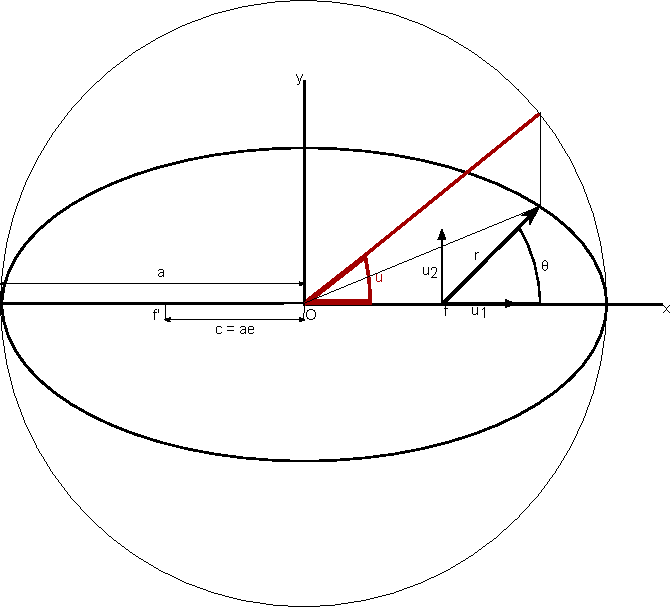
\includegraphics{eliptica}
\par\end{centering}

\caption{\label{fig:elementoselip}Elementos de la órbita elíptica}
\end{figure}


Siendo $\vec{\mathbf{e}}\:$el origen de ángulos de la anomalía verdadera,
pueden deducirse fácilmente los radios del pericentro y apocentro
en las posiciones $\theta=0\:$y $\theta=180\:$respectivamente
\begin{gather}
r_{p}\:=\:\frac{p}{1+e}\\
r_{a}\:=\:\frac{p}{1-e}
\end{gather}


y por tanto, el eje mayor de la elipse
\begin{equation}
2a\:=\: r_{a}+r_{p}\:=\:\frac{2p}{1-e^{2}}
\end{equation}


En estos ejes perifocales queda descrita la trayectoria por medio
de las ecuaciones
\begin{equation}
\begin{array}{c}
x\:=\: r\cdot cos\theta\\
y\:=\: r\cdot sen\theta\\
z\:=\:0
\end{array}\label{eq:posorbper}
\end{equation}
y la velocidad $\vec{\mathbf{v}}$(A partir de \ref{eq:trayectoriaelip},\ref{eq:posorbper}
y la primera fórmula de Binet)
\begin{equation}
\begin{array}{c}
v_{x}\:=\:-\frac{\mu}{h}sen\theta\\
v_{y}\:=\:\frac{\mu}{h}(e+cos\theta)\\
v_{z}\:=\:0
\end{array}
\end{equation}


Puede resultar conveniente en algunos casos describir la trayectoria
no tomando como origen el foco ocupado, sino el centro geométrico
de la elipse O (Ver Figura \ref{fig:elementoselip}). Se toman los
ejes paralelos a los ejes perifocales, pero con origen en el centro
geométrico y se imagina una circunferencia de radio a, sobre la que
se proyecta (según el eje y) la posición de la partícula. En este
caso, el ángulo u que forma el radiovector con el eje x se denomina
\emph{anomalía excéntrica }y sirve para describir la trayectoria en
este nuevo sistema de ejes de manera muy sencilla con los dos semiejes
de la órbita.
\begin{equation}
\begin{array}{c}
x\:=\: a\cdot cos\, u\\
y\:=\: b\cdot sen\, u\\
z\:=\:0
\end{array}
\end{equation}


El cambio entre ambos sistemas se realiza de manera fácil mediante
las ecuaciones
\begin{alignat}{1}
sen\theta\:=\:\frac{\sqrt{1-e^{2}}sen\, u}{1-e\, cos\, u} & \qquad cos\theta\:=\:\frac{cos\, u-e}{1-e\, cos\, u}
\end{alignat}


o sus inversas
\begin{align}
sen\, u\:=\:\frac{\sqrt{1-e^{2}}sen\theta}{1+e\, cos\theta} & \qquad cos\, u\:=\:\frac{cos\theta+e}{1+e\, cos\theta}
\end{align}


La anomalía excéntrica sirve también como paso intermedio para calcular
la ley horaria del movimiento. Hasta ahora tenemos una relación $r\:=\: r(\theta)\:$,
de manera que para determinar $r\:=\: r(t)\:$ necesitamos $\theta(t)$.
A esta última relación se la llama \emph{ley horaria}. Apoyándose
en la segunda ley de Kepler y en distintas propiedades geométricas,
puede demostrarse que
\begin{equation}
M\:=\: n(t-\tau)\:=\: u-e\, sen\, u
\end{equation}


con $n=\frac{2\pi}{T}\:$ la velocidad angular media y $\tau\:$ el
tiempo de paso de la partícula por el pericentro. A esta ecuación
se la conoce como \emph{ecuación de Kepler} y, salvo casos particulares,
debe resolverse numéricamente.


\section{Elementos clásicos de la órbita}

El problema de una partícula orbitando alrededor de un cuerpo central
queda unequivocamente determinado por 6 parámetros. Estos parámetros
son típicamente la posición y velocidad de la partícula en un instante
determinado, normalmente el inicial, y a partir de esas 3+3 componentes
puede determinarse la posición que ocupará el objeto en cualquier
otro instante de tiempo. Sin embargo, en numerosas ocasiones resulta
más conveniente y cómodo usar otro conjunto de parámetros llamados
elementos clásicos de la órbita, que simpplifican mucho el cálculo
de la posición y velocidad de la partícula. Estos elementos típicamente
son:
\begin{itemize}
\item \emph{El semieje mayor }\textbf{\emph{a}}, que da una idea del tamaño
de la órbita
\item \emph{La excentricidad }\textbf{\emph{e}}, que indica la forma de
la órbita
\item \emph{La longitud recta del nodo ascendente }\textbf{\emph{Ω}}\emph{,
la inclinación }\textbf{\emph{i }}\emph{y el argumento del perigeo
}\textbf{\emph{ω}}\emph{, }una serie de giros consecutivos que permiten
situar el plano de la órbita en el espacio.
\item \emph{La anomalía verdadera }\textbf{\emph{θ}}, que situa la partícula
dentro de su órbita. Este parámetro puede ser sustituido por otro
equivalente, como la anomalía excentrica o el tiempo de paso por el
perigeo
\end{itemize}
\begin{figure}
\begin{centering}
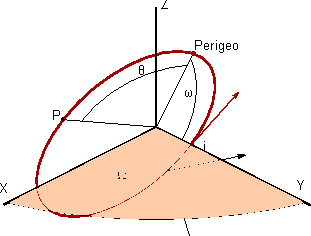
\includegraphics{elementosclasicos}
\par\end{centering}

\caption{\label{fig:elementosorbita}Elementos clásicos de la órbita}
\end{figure}


La determinación de estos elementos a partir de la posición $\vec{\mathbf{r}}\,$y
velocidad $\vec{\mathbf{v}}\,$en un punto se hace de manera fácil
mediante el siguiente algoritmo
\begin{itemize}
\item Determinación de $\vec{\mathbf{h}}\,$y $\vec{\mathbf{e}}$
\[
\vec{\mathbf{h}}\:=\:\vec{\mathbf{r}}\times\vec{\mathbf{v}}
\]
\[
\vec{\mathbf{e}}\:=\:-\frac{\vec{\mathbf{r}}}{r}-\frac{1}{\mu}(\vec{\mathbf{h}}\times\vec{\mathbf{v}})
\]

\item Determinación de la referencia perifocal y la dirección del nodo ascendente
\[
\begin{array}{cc}
\vec{\mathbf{u_{1}}}\:=\:\frac{\vec{\mathbf{e}}}{e}\qquad & \vec{\mathbf{u_{3}}}\:=\:\frac{\vec{\mathbf{h}}}{h}\\
\vec{\mathbf{u_{2}}}\:=\:\vec{\mathbf{u_{3}}}\times\vec{\mathbf{u_{1}}}\qquad & \vec{\mathbf{n_{1}}}\:=\:\frac{\vec{\mathbf{k}}\times\vec{\mathbf{u_{3}}}}{\left|\vec{\mathbf{k}}\times\vec{\mathbf{u_{3}}}\right|}
\end{array}
\]

\item Determinación de los elementos de la órbita
\begin{equation}
\begin{array}{cc}
cos\,\Omega\:=\:\vec{\mathbf{n_{1}}}\cdot\vec{\mathbf{i}} & \qquad sen\,\Omega\:=\:\vec{\mathbf{n_{1}}}\cdot\vec{\mathbf{j}}\\
\\
cos\,\omega\:=\:\vec{\mathbf{u_{1}}}\cdot\vec{\mathbf{n_{1}}} & \qquad sen\,\omega\:=\:(\vec{\mathbf{n_{1}}}\times\vec{\mathbf{u_{1}}})\cdot\vec{\mathbf{u_{3}}}\\
\\
cos\, i\:=\text{\:}\vec{\mathbf{u_{3}}}\cdot\vec{\mathbf{k}}\\
\\
e\:=\:\left|\vec{\mathbf{e}}\right|\\
\\
a=\frac{p}{1-e^{2}}\\
\\
cos\,\theta\:=\:\vec{\mathbf{r}}\cdot\vec{\mathbf{u_{1}}} & sen\,\theta\:=\:\vec{\mathbf{r}}\cdot\vec{\mathbf{u_{2}}}
\end{array}\text{}
\end{equation}

\end{itemize}

\section{Cuaternios}

Ya se ha visto que manejar los elementos clásicos de la órbita implica
considerar cuatro giros distintosa la hora de calcular una posición
respecto a los ejes de referencia, y además estos giros deben realizarse
en un orden concreto y preciso. Por si fuera poco, otras aplicaciones
a otros problemas mecánicos pueden encontrar conveniente usar otra
secuencia de giros para describir su estado. Es por ello que se necesita
una manera de tratar de forma matématica esta serie de movimientos
concatenados, y que dicha manera sea fiable y barata computacionalmente
hablando.

Si pensamos en un vector $\vec{\mathbf{u}}$, descompuesto en sus
coordenadas cartesianas en un sistema de ejes ($\begin{array}{ccc}
\vec{\mathbf{i}} & \vec{\mathbf{j}} & \vec{\mathbf{k}}\end{array}$) de manera que $\vec{\mathbf{u}}\:=\: u_{1}\vec{\mathbf{i}}+u_{2}\vec{\mathbf{j}}+u_{3}\vec{\mathbf{k}}\:$,
podemos expresar el vector $\vec{\mathbf{u}}\,$ en otro sistema de
ejes resultado de aplicar un giro de θ grados alrededor de, por ejemplo,
el eje z mediante las ecuaciones
\[
\begin{array}{c}
u'_{1}\:=\: u_{1}\cdot cos\,\theta+u_{2}\cdot sen\,\theta\\
u'_{2}\:=\:-u_{1}\cdot sen\,\theta+u_{2}\cdot cos\,\theta\\
u'_{3}\:=\: u_{3}
\end{array}
\]
o, escribiéndolo de forma matricial
\[
\left(\begin{array}{c}
u'_{1}\\
u'_{2}\\
u'_{3}
\end{array}\right)\:=\:\left(\begin{array}{ccc}
cos\,\theta & sen\,\theta & 0\\
-sen\,\theta & cos\,\theta & 0\\
0 & 0 & 1
\end{array}\right)\cdot\left(\begin{array}{c}
u_{1}\\
u_{2}\\
u_{3}
\end{array}\right)\:=\: R\cdot\vec{\mathbf{u}}
\]


A la matriz \emph{R} se la denomina \emph{matriz de cambio de base},
y su cálculo es sencillo, además de que el giro es aparente a primera
vista. La operación de cambio de base también es sencilla y se puede
realizar con papel y lápiz rápidamente. El proceso se complica cuando
se concatenan varios giros seguidos, ya que al multiplicar las matrices
pierden su forma tan regular. Sin embargo, hay que considerar que
el ordenador realiza el mismo número de operaciones haya un 0 u otro
número, introduciendo errores con cada operación, y también tiene
que almacenar los 9 números que contiene la matriz. Es por esta razón
por la que, en aplicaciones informáticas, se prefiera y resulta más
eficiente el empleo de los denominados cuaternios.


\subsubsection{Definición y operaciones}

Se define un cuaternio como una extensión a los números reales, un
conjunto de 4 números que siguen una serie de reglas definidas, y
suelen expresarse de manera
\[
\mathbf{q}\:=\: q_{0}+q_{1}\cdot i+q_{2}\cdot j+q_{3}\cdot k
\]
A $q_{0}\,$se le denomina parte real y al conjunto de componentes
$q_{1},\, q_{2}\, y\, q_{3}\:$ se le llama parte imaginaria. Se definen
la suma y el producto de manera parecida a los números complejos,
teniendo cuidado de no mezclar las distintas componentes. Para los
distintos productos cruzados, puede usarse la siguiente tabla, eligiendo
el primer factor del producto entre las filas y el segundo entre las
columnas.
\begin{equation}
\begin{array}{cccccc}
 &  & 1 & i & j & k\\
\\
1 &  & 1 & i & j & k\\
i &  & i & -1 & k & -j\\
j &  & j & -k & -1 & i\\
k &  & k & j & -i & -1
\end{array}
\end{equation}
Merece especial mención el hecho de que el producto entre dos cuaternios
no es conmutativo.

Se define el cuaternio conjugado $\bar{\mathbf{q}}\:$ como aquel
con la misma parte real pero parte imaginaria cambiada de signo (Las
tres componentes). Se define la norma de $\mathbf{q}\:$como el producto
$\left|\mathbf{q}\right|\:=\text{\:}\sqrt{\mathbf{q}\cdot\bar{\mathbf{q}}}\:=\:\sqrt{q_{0}^{2}+q_{1}^{2}+q_{2}^{2}+q_{3}^{2}}$.
Nótese que el producto del interior de la raiz da siempre como resultado
un número real, y por tanto se aplica la definición de raiz clásica.
Así mismo, se llama \emph{cuaternio unitario }a aquel que tiene norma
unidad.


\subsubsection{Cuaternios vectoriales}

Del mismo modo que los números complejos resultan muy útiles a la
hora de describir y operar con vectores en el plano, los cuaternios
pueden usarse para los mismos fines en el espacio $\mathbb{R^{\mathit{\textrm{3}}}}$.
Se llama cuaternio vectorial a un cuaternio con parte real nula, de
manera que las tres componentes de la parte imaginaria coinciden con
las componentes de un vector.

Si se tiene un cuaternio unitario $\mathbf{c}$, de manera que $c_{0}^{2}+c_{1}^{2}+c_{2}^{2}+c_{3}^{2}\:=\:1$,
puede hacerse un cambio de variable
\begin{gather*}
cos\,\frac{\theta}{2}\:=\: c_{0}\\
sen\,\frac{\theta}{2}\:=\:\sqrt{c_{1}^{2}+c_{2}^{2}+c_{3}^{2}}\\
\vec{\mathbf{e}}\:=\:\frac{c_{1}}{sen\,\frac{\theta}{2}}\vec{\mathbf{i}}+\frac{c_{2}}{sen\,\frac{\theta}{2}}\vec{\mathbf{j}}+\frac{c_{3}}{sen\,\frac{\theta}{2}}\vec{\mathbf{k}}
\end{gather*}
el cuaternio \textbf{c} puede expresarse de manera
\begin{equation}
\mathbf{c}\:=\: cos\,\frac{\theta}{2}+sen\,\frac{\theta}{2}\vec{\mathbf{e}}
\end{equation}
y el cuaternio \textbf{c} queda perfectamente definido unequivocamente
por el par $(\theta,\vec{\mathbf{e}})$.

Puede demostrarse entonces que la operación
\begin{equation}
\vec{\mathbf{v}}\:=\:\mathbf{c}\cdot\vec{\mathbf{u}}\mathbf{\cdot}\bar{\mathbf{c}}\label{eq:girocuaternios}
\end{equation}
corresponde a un giro del vector $\vec{\mathbf{u}}$, θ grados alrededor
de la dirección $\vec{\mathbf{e}}$.

Usar esta operación presenta muchas ventajas frente al empleo de matrices
de giro. Al ser el cuaternio \textbf{c} unitario, la relación inversa
es obtenible inmediatamente sin más que multiplicar ambos lados de
la ecuación \ref{eq:girocuaternios} por $\bar{\mathbf{c}}\,$y \textbf{c}
por la izquierda y derecha respectivamente, sin necesidad de la costosa
operación de calcular la inversa de una matriz. Los cuaternios puede
concatenarse de manera parecida a las matrices, mediante un producto
directo, teniendo cuidado con el orden de los factores. Y por último,
únicamente requieren almacenar 4 parámetros, en lugar de los 9 de
la matriz. Es por todas estas razones que, en aplicaciones informáticas,
resulta conveniente usar este sistema para realizar todos los giros
necesarios.


\section{Perturbaciones}


\subsection{Tierra esférica}

La esfericidad de la tierra se conoce desde tiempos antiguos. Ya en
el siglo III a.C. el astrónomo griego Eratóstenes dio una primera
aproximación numérica del radio de la tierra con una precisión espectacular
para la época, midiendo la distancia entre Siena y Alejandría y el
ángulo que formaba la sombra del sol el mismo día en ambas ciudades.
Esta medida se ha ido refinando con distintas observaciones posteriores
hasta el valor del radio medio de 6371.0 Km que se maneja hoy en día.
Así, es posible hacer una primera aproximación de la tierra
\begin{figure}
\begin{centering}
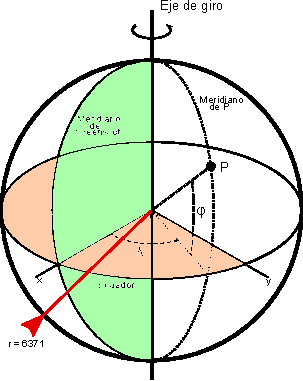
\includegraphics{tierraesferica}
\par\end{centering}

\caption{Tierra esférica\label{fig:Tierra-esf=0000E9rica}}
\end{figure}


Se define la longitud como el ángulo que forma el meridiano que pasa
por el punto P con el meridiano de referencia que pasa por Greenwich.
La longitud en grados está en el intervalo {[}-180,180{]}, siendo
positiva al este de Greenwich y negativa al oeste. Se define de manera
precida la latitud, siendo el ángulo que forma el radiovector que
une el centro de la tierra con el punto P con el radiovector que une
el centro con el punto que está a la vez en el meridiano de P y en
el ecuador. La latitud está contenida en {[}-90,90{]} grados, siendo
positiva para el hemisferio norte y negativa para el hemisferio sur.

Sin embargo, unido a la mejora de la precisión en la medida del radio
de la tierra, se ha descubierto que la tierra no tiene forma ésferica.
El valor de 6371.0 no es el radio verdadero, sino una media calculada
a través de modelos más precisos. La corrección más importante al
modelo esférico es el achatamiento terrestre. La tierra es un planeta
\emph{oblato}, con un radio ecuatorial mayor que el radio en los polos.
Esto es debido principalmente a la rotación de la tierra y las fuerzas
de inercia que se producen. Una vez descartamos la aproximación esférica,
la siguiente figura geométrica que aproxima mejor la tierra es un
elipsoide.

Se define un cuerpo de revolución, con sección elíptica, de manera
que todas las secciones que contienen al eje de revolución son iguales.
Como elípse, se usan los parámetros geométricos típicos \emph{a, b,
e=c/a} (semiejes mayor, menor y excentricidad respectivamente) y,
por comodidad, se define un parámetro extra llamado \emph{achatamiento
\[
f\:=\text{\:}\frac{a-b}{b}
\]
\[
e^{2}\:=\: f\cdot(2-f)
\]
}

Los valores de estos párametros han ido recibiendo, de nuevo, más
precisión a medida que se recogían datos. Uno de los modelos más aceptados
hoy en día, y el que usa el programa, es el \textbf{WGS84} (World
Geodetic System 1984). Este sistema, aunque comprende modelos más
complejos, da valores para un elipsoide
\begin{gather*}
Semieje\: mayor\quad a\:=\:6378.137\, Km\\
Inverso\: achatamiento\quad\frac{1}{f}\:=\text{\:}298.257223563
\end{gather*}


El introducir el elipsoide conlleva complejidad adicional a calcular
el valor del radio. Se define la \emph{latitud geodésica} $\varphi_{g}$
como el ángulo que forma la vertical local por P con el plano del
ecuador, mientras que la \emph{latitud geocéntrica $\varphi_{c}$}
coincide con la definición anterior. La latitud geodésica es la que
aparece en los mapas y la que se usa para georeferenciar un punto.
\begin{figure}
\begin{centering}
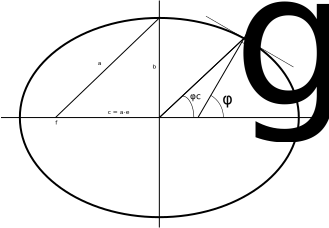
\includegraphics{elipsoide}
\par\end{centering}

\caption{\label{fig:Elipsoide-de-referencia}Sección del elipsoide de referencia}
\end{figure}


Las ecuaciones de la elipse en función de la latitrud geodésica son
\begin{equation}
\begin{array}{c}
x_{P'}\:=\:\frac{a\cdot cos\,\varphi_{g}}{\sqrt{1-e^{2}sen^{2}\varphi_{g}}}\\
\\
z_{P'}\:=\text{\:}\frac{a(1-e^{2})sen\,\varphi_{g}}{\sqrt{1-e^{2}sen^{2}\varphi_{g}}}
\end{array}\label{eq:geodesica}
\end{equation}
mientras que la latitud geocéntrica cumple
\begin{equation}
\begin{array}{c}
cos\,\varphi_{c}\:=\:\frac{x_{P'}}{\sqrt{x_{P'}^{2}+z_{P'}^{2}}}\\
\\
sen\,\varphi_{c}\:=\:\frac{z_{P'}}{\sqrt{x_{P'}^{2}+z_{P'}^{2}}}
\end{array}\label{eq:geocentrica}
\end{equation}


Para un punto cualquiera del espacio, con la ecuación de la recta
normal al elipsoide y las ecuaciones anteriores se obtiene
\begin{equation}
x\cdot sen\varphi_{g}-zcos\,\varphi_{g}-a\frac{e^{2}\cdot sen\,\varphi_{g}\cdot cos\varphi_{g}}{\sqrt{1-e^{2}sen^{2}\varphi_{g}}}\:=\:0
\end{equation}
ecuación que ha de resolverse numéricamente para $\varphi_{g}$. Como
primer paso en el proceso iterativo, pueden aproximarse las ecuaciones
\ref{eq:geodesica} y \ref{eq:geocentrica} para obtener 
\[
\varphi_{g}\:\thickapprox\:\varphi_{c}+\frac{e^{2}}{2}sen\,2\varphi_{c}
\]


El modelo completo WGS84 no incluye únicamente la definición de un
elipsoide de referencia, sino que contempla una figura mucho más compleja
y mucho más cercana a la realidad llamada \emph{geoide}. El geoide
no se define de la misma manera que los dos modelos anteriores, a
partir de una figura geométrica, sino que es una \emph{superficie
equipotencial del campo gravitatorio terrestre}, teniendo en cuenta
la fuerza de inercia de la rotación de la tierra y todos los armónicos
de la gravedad. Las medidas de distintas misiones espaciales han permitido
generar modelos tan complejos como la figura \ref{fig:Geoide}%
\footnote{Imagen obtenida a partir de los datos de la misión GOCE de la ESA,
que pueden encontrarse en https://earth.esa.int/web/guest/missions/ %
}
\begin{figure}
\begin{centering}
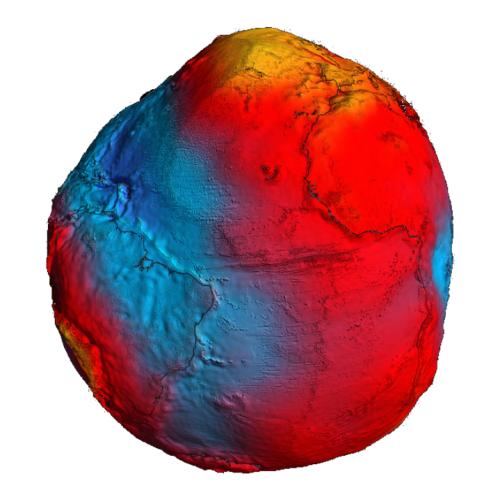
\includegraphics{geoide}
\par\end{centering}

\caption{Geoide\label{fig:Geoide}}
\end{figure}


Este último modelo escapa a la complejidad y precisión del programa,
por lo que se usará la definición del elipsoide.


\subsection{Campo gravitatorio}

La fórmula de la gravitación universal \ref{eq:gravitacionuniversal}
ha asumido que las dos partículas que interaccionan son masas puntuales,
objetos ficticios con toda su masa concentrada en un único punto adimensional.
Sin embargo, ni la tierra es un objeto puntual ni, dentro de su forma
geométrica vista en el apartado anterior, toda su masa está distribuida
de manera uniforme. Esto lleva a que el campo gravitatorio que genera
no sea tan sencillo como la aproximación esférica supone.

Se define un campo escalar conservativo llamado potencial, como el
trabajo que realiza la fuerza gravitatoria por unidad de masa, de
manera que 
\[
U\:=\text{\:}\int_{r_{ref}}^{r}g\cdot\mathrm{d}r
\]
y
\begin{equation}
g\:=\:-\nabla U
\end{equation}
En el caso de un campo esférico obtenemos
\begin{equation}
U\:=\: GM\int_{\infty}^{r}\frac{1}{r^{2}}\,\mathrm{d}r\:=\:-\frac{GM}{r}
\end{equation}
pero esta aproximación sólo resulta adecuada para un cuerpo esférico.


\subsubsection{Cuerpo casi esférico}

Podemos considerar que un cuerpo no esférico está compuesto por infinitas
masas puntuales de manera que 
\[
dU\:=\text{\:}\frac{G}{r'}dM
\]
y el potencial total será la suma de cada uno de estos potenciales
a lo largo y angho de todo el cuerpo. Un tratamiento típico de esta
ecuación es desarollarla en una serie de armónicos esféricos, de manera
que se obtiene
\begin{equation}
U\:=\text{\:}-\frac{G}{r}\int\mathrm{d}M-\frac{G}{r^{2}}\int s\, cos\,\varphi\,\mathrm{d}M-\frac{G}{r^{3}}\int s^{2}\mathrm{d}M+\frac{3}{2}\frac{G}{r^{3}}\int s^{2}sen^{2}\varphi\,\mathrm{d}M+...\label{eq:potencialserie}
\end{equation}


Una primera aproximación consiste en suponer que el cuerpo es un cuerpo
casi esférico, es decir, un cuerpo de revolución con una generatriz
no circular, de manera que sus momentos principales de inercia $A\:=\text{\:}B\:\neq\: C$
que permite escribir la ecuación \ref{eq:potencialserie}, mediante
la fórmula de MacCullagh como
\begin{gather}
U\:=\:-\frac{GM}{r}+\frac{GJ_{2}Ma^{2}}{r^{3}}(\frac{3}{2}cos^{2}\varphi-\frac{1}{2})\\
J_{2}\:=\:\frac{C-A}{Ma^{2}}\nonumber 
\end{gather}
y de está ecuación puede derivarse con facilidad en coordenadas rectangulares
\begin{gather*}
\vec{\mathbf{g}}\:=\:-\mathbf{\nabla}U\:=\:\left(\begin{array}{c}
-\frac{GM}{r^{3}}x\\
\\
-\frac{GM}{r^{3}}y\\
\\
-\frac{GM}{r^{3}}z
\end{array}\right)+\left(\begin{array}{c}
\frac{-3C\cdot x\cdot(1-5(\frac{z}{r})^{2})}{r^{5}}\\
\\
\frac{-3C\cdot y\cdot(1-5(\frac{z}{r})^{2})}{r^{5}}\\
\\
\frac{-3C\cdot z\cdot(3-5(\frac{z}{r})^{2})}{r^{5}}
\end{array}\right)\\
C\:=\:\frac{J_{2}GMa^{2}}{2}
\end{gather*}


El modelo \textbf{JGM 3} (Joint Gravitational Model) da un valor %
\footnote{http://www.csr.utexas.edu/publications/statod%
} para el parámetro $J_{2}\:=\:1.082636\cdot10^{-3}$


\subsubsection{Armónicos esféricos}

Hasta el momento se ha considerado únicamente el achatamiento terrestre.
Pero, aunque es el más importante, no es el único efecto de perturbación
sobre el campo gravitatorio. Puede seguir desarrollándose el potencial
en una serie de armónicos esféricos, de manera que cumpla la ecuación
de Laplace $(\nabla^{2}U\:=\:0)$ como
\begin{equation}
U\:=\:-[\frac{\mu}{r}+\frac{\mu}{r}\sum\frac{J_{n}P_{n}^{0}}{(\frac{r}{a})^{n}}_{n=2}^{N}+\frac{\mu}{r}\sum_{n=2}^{N}\sum_{m=0}^{n}P_{n}^{m}(C_{n}^{m}cos\, m\theta+S_{n}^{m}sen\, m\theta)]
\end{equation}


Donde se han separado en otro sumando los términos simétricos en $\varphi$.
Los diversos $P_{n}^{m}\,$se conocen como polinomios y funciones
de Legendre, y están muy documentados y desarollados en diversas fuentes
hasta un alto orden. Los distintos coeficientes $J_{n},\, C_{n}^{m}\, y\, S_{n}^{m}\,$vienen
dados en varios modelos empíricos. Uno de los más usados es el \textbf{EGM96}
(Earth Gravitational Model 1996), que engloba el usado JGM3. %
\footnote{Los coeficientes hasta orden 360 pueden encontrarse en http://cddis.gsfc.nasa.gov/egm96/getit.html%
} 

Este análisis detallado escapa de nuevo al rango del programa, que
únicamente usará el término esférico y su perturbación mayor, $J_{2}$


\subsection{Atmósfera}

La carácterística principal del espacio es que está \emph{vacio},
un gran vacio con pequeñas agrupaciones locales de materia que llamamos
estrellas, planetas, asteroides y demás astros que pueblan el universo.
Y aunque este hecho no es del todo cierto, lo es menos aún cuando
nos referimos a los alrededores de un astro con atmósfera. ¿Donde
está el límite entre la atmósfera y el vacio? Lo cierto es que poner
una frontera es muy difícil, y es más adecuado tratar la atmósfera
como algo continuo. Esta presencia de atmósfera afecta a los satélites
en forma de resistencia aerodinámica, de manera similar a los aviones
volando en la estratosfera.

La resistencia aerodinámica es fácilmente la perturbación más complicada
de calcular de todas aquellas que afecta a los satélites que orbitan
la tierra. El modelo más sencillo que podemos pensar es
\begin{equation}
\vec{\mathbf{a_{atm}}}\:=\:-\frac{1}{2}\frac{C_{D}A_{f}}{m}\rho v_{w}^{2}\cdot\frac{\mathbf{\vec{v_{w}}}}{v_{w}}
\end{equation}
El cálculo de las distintas variables implicadas, no demasiado complicado
cuando se trata de vuelo atmósferico, se dispara en el caso de satélites
con mucha complejidad.


\subsubsection{Velocidad relativa $\mathbf{\vec{v_{w}}}$}

A priori es el parámetro más sencillo de calcular, pero debido al
poco conocimiento que hay del movimiento de las capas altas de la
atmósfera su precisión no será muy alta. Suponiendo que la atmósfera
está fija a la tierra y gira con ella, se tiene
\begin{equation}
\mathbf{\vec{v_{w}}}\:=\:\mathbf{\vec{v_{sat}}}-\vec{\mathbf{\omega_{T}}}\times\vec{\mathbf{r}}
\end{equation}



\subsubsection{Área frontal $A_{f}$, coeficiente de resistencia $C_{D}$}

El cálculo del coeficiente de resistencia se complica mucho frente
al del vuelo atmosférico. A altas altitudes, el camino medio del flujo
de aire comienza a ser del orden de los tamaños de los sólidos volando
a través de él, y por tanto las hipótesis de flujo continuo dejan
de ser válidas. Es necesario calcular ahora el flujo como un choque
de particulas sueltas, con choques más o menos elásticos y difusos
dependiendo de las propiedades de la superficie y de su orientación.
Además, por la dificultad de tomar muestras, se dispone de muy pocos
datos experimentales que sirvan para refinar y corregir estos modelos.

El área frontal también puede ser un problema, ya que no siempre es
fácil conocer con precisión la actitud de un satélite frente al flujo.
La geometría suele ser complicada, con grandes elementos como paneles
o antenas extendidos y muchas partes de la estructura expuestas directamente
al flujo.

La manera más fácil de tratar todos estos parámetros es agruparlos
en un único valor, llamado \emph{coeficiente balístico}, y definido
como
\begin{equation}
CB\:=\:\frac{m}{C_{D}A_{f}}
\end{equation}
aunque a veces se usa la relación inversa. La precisión de la fuerza
de resistencia dependerá de la precisión con la que se sea capaz de
expresar el CB. Valores típicos del coeficiente balístico rondan en
el intervalo {[}20,50{]}, dependiendo del tamaño del satélite. El
programa usa un modelo de CB constante, para evitar la complejidad
y la cantidad de datos previos necesarios que habría que calcular
en caso de querer determinar con más exactitud este valor.


\subsubsection{Densidad $\rho$}

El cálculo de la densidad es complejo, porque los modelos que se tienen
están basados en datos y correcciones empíricas y no se tienen muy
claros y detallados todos los fenómenos que influyen en este parámetro.
Se sabe que el sol sufre un ciclo en su emisión de radiación lo largo
de unos 11 años, que afecta directamente a la atmósfera haciendo que
``engorde'' o ``adelgace'' según la actividad sea mayor o menor.
Esta emisión suele concretarse en el índice $F_{10,7}$, que es una
medida de las emisiones del sol en la longitud de onda de 10.7cm,
y que resulta muy conveniente ya que se tienen gran cantidad de datos
de su comportamiento a lo largo de mucho tiempo%
\footnote{Datos sobre el flujo actual y un historial pueden encontrarse en http://www.swpc.noaa.gov/phenomena/f107-cm-radio-emissions%
}. Otro parámetro común que usan algunos modelos es la temperatura
exoesférica, $T_{\infty}$, que es una medida indirecta del mismo
fenómeno. El programa usa una temperatura exosférica fija que corresponde
a una media a lo largo del ciclo solar, $T_{\infty}\:=\:1000K$

La variación de la densidad con la altura no es menos compleja, ya
que, a diferencia de la atmósfera cercana, la toma de datos es complicada
y esporádica. La composición de la atmósfera cambia y aparecen especies
que no se dan en las capas bajas y que reaccionan de manera distinta
a distintas frecuencias de radiación. Distintos modelos han tratado
de representar todos estos fenómenos, cada uno trabajando sobre el
anterior con nuevos datos para mejorar su precisión. Uno de ellos,
el que usa el programa, es el \textbf{Jacchia 1977}, que da los distintos
datos de densidad, temperatura y presión de las especies más comunes
en un rago de alturas muy amplio cada Km, a partir de los cuales se
obtienen en el resto de alturas por simple interpolación lineal. El
hecho de tener esta estructura tabular hace que el algoritmo sea complejo
y farragoso de reproducir aqui, pero puede encontrarse íntegro, junto
con muchos modelos más, en \emph{http://nssdcftp.gsfc.nasa.gov/models/}


\section{Integración numérica}

Ya hemos visto la solución analítica del problema de los dos cuerpos
sin perturbar, pero la introducción de otras fuerzas con distintas
formas matemáticas complica el problema bastante, hasta el punto en
que resulte imposible hayar una solución sencilla. En este momento,
es cuando se justifica la introducción de otro tipo de solución, una
solución numérica. La elección del método numérico resulta fundamental
a la hora de obtener una buena precisión en la solución. El método
no sólo debe ser preciso, sino que además debe ser estable, propiedad
que depende tanto del método numérico como del problema específico
al que se aplica y del paso de integración que se elija. Por esta
importancia, el programa deja elegir entre varios integradores y definir
el paso a la hora de plantear las condiciones iniciales.

La ecuación \ref{eq:newton2} ampliada con las fuerzas de perturbación
puede escribirse en términos
\begin{equation}
\vec{\ddot{\mathbf{x}}}\:=\: F(t,\vec{\mathbf{x}},\vec{\dot{\mathbf{x}}})\:=\:-\frac{\mu}{r^{3}}\vec{\mathbf{r}}+\vec{\mathbf{F_{p}}}
\end{equation}
Que es una ecuación diferencial de segundo orden. Definiendo un vector
\begin{equation}
\mathbf{y}\:=\:\left\{ \vec{\mathbf{x}},\vec{\dot{\mathbf{x}}}\right\} 
\end{equation}
puede escribirse
\begin{equation}
\dot{\mathbf{y}}\:=\: f(t,\mathbf{y})
\end{equation}
de manera que ahora se trata de un problema de primer orden, linealizable
e integrable numéricamente. La función \emph{f }puede descomponerse
en dos términos según la forma de sus distintas componentes
\[
\dot{\mathbf{y}}\:=\:\left(\begin{array}{c}
\vec{\dot{\mathbf{x}}}\\
\vec{\ddot{\mathbf{x}}}
\end{array}\right)\:=\:\left(\begin{array}{cc}
0 & 1\\
F_{x} & F_{\dot{x}}
\end{array}\right)\cdot\left(\begin{array}{c}
\vec{\mathbf{x}}\\
\vec{\dot{\mathbf{x}}}
\end{array}\right)+\left(\begin{array}{c}
0\\
\vec{\mathbf{F}}
\end{array}\right)\:=\:\mathbb{\mathtt{A}}\cdot\mathbf{y}+b
\]
Donde en la matriz aparecen los términos de las fuerzas que dependen
linealmente de $\vec{\mathbf{x}}\;$y$\vec{\dot{\mathbf{x}}}\;$respectivamente,
y en \emph{b} el resto de fuerzas implicadas. El análisis de la matriz
\textbf{A} permite determinar el rango de soluciones donde el metodo
será estable, pero en este caso, al no haber fuerzas lineales, toma
la forma $\mathtt{A}\:=\text{\:}\left(\begin{array}{cc}
0 & 1\\
0 & 0
\end{array}\right)\:$y todas las fuerzas aparecen en el término independiente. 

La integración numérica consiste en sustituir la solución analítica,
que tiene forma de ecuación más o menos complicada, por una solución
que está definida en una serie de puntos y sólo en ellos. La solución
toma la forma de una lista de puntos, separados por lo que se conoce
como el paso de integración. Aprovechándose de la continuidad de la
solución y sus derivadas, se usa un punto (O varios) $\mathbf{y}_{n}\;$anterior
para calcular la solución en el punto nuevo $\mathbf{y}_{n+1}$. Dependiendo
del método que se elija, se necesitan más o menos valores anteriores
para hallar esta nueva solución.


\subsubsection{Runge-Kutta}

Esta familia de métodos se caracteriza por ser de paso simple, es
decir, por necesitar únicamente el último paso de integración para
calcular el siguiente. El aumento de precisión respecto al método
de Euler consiste en evaluar las derivadas de orden más alto a través
de la evaluación de \emph{f} en distintos puntos. Uno de los más usados
es el de cuarto orden definido por
\begin{gather}
\mathbf{y}_{n+1}\:=\:\mathbf{y}_{n}+\frac{\triangle t}{6}(\mathbf{k}_{1}+2\mathbf{k}_{2}+2\mathbf{k}_{3}+\mathbf{k_{4}})\nonumber \\
\mathbf{k}_{1}\:=\: f(t_{n},\mathbf{y}_{n})\nonumber \\
\mathbf{k}_{2}\:=\: f(t_{n}+\frac{\triangle t}{2},\mathbf{y}_{n}+\frac{\triangle t}{2}\mathbf{k}_{1})\\
\mathbf{k}_{3}\:=\: f(t_{n}+\frac{\triangle t}{2},\mathbf{y}_{n}+\frac{\triangle t}{2}\mathbf{k}_{2})\nonumber \\
\mathbf{k}_{4}\:=\: f(t_{n}+\triangle t,\mathbf{y}_{n}+\triangle t\mathbf{k}_{3})\nonumber 
\end{gather}



\subsubsection{Adams-Bashforth}

Esta familia de métodos se caracterizan por ser multipaso, por usar
varias soluciones anteriores para calcular un paso determinado, y
por ser explicitos, es decir, porque la solución del nuevo paso depende
únicamente de las soluciones en los puntos anteriores, y no de la
solución nueva desconocida. El método Adams-Bashforth de cuarto orden
consiste en
\begin{equation}
\mathbf{y}_{n+1}\:=\:\mathbf{y}_{n}+\frac{\triangle t}{24}(55\, f_{n}-59\, f_{n-1}+37\, f_{n-2}-9\, f_{n-3})
\end{equation}
Naturalmente este método requiere conocer la solución en cuatro puntos
anteriores, por lo que debe iniciarse con otro método de paso simple
hasta tener el número requerido. En caso de seleccionarse este método,
el programa usa el Runge-Kutta de cuarto orden para hallar los cuatro
primeros puntos.


\subsubsection{Adams-Moulton}

Esta es una familia de métodos multipaso implicitos, ya que la solución
en el nuevo paso cumple un papel en la ecuación que determina esa
misma solución. Se debe disponer antes, por tanto, de una estimación
de la nueva solución antes de poder aplicar este método. El Adams-Moulton
de cuarto orden consiste en
\begin{equation}
\mathbf{y}_{n+1}\:=\:\mathbf{y}_{n}+\frac{\triangle t}{24}(9\, f_{n+1}+19\, f_{n}-5\, f_{n-21}+f_{n-2})
\end{equation}


Como estimador para calcular $f_{n+1}\:$puede usarse cualquiera de
los métodos anteriores. En el caso del programa, se trata del Adams-Bashforth
de cuarto orden.


\subsubsection{Predictor-Corrector}

El uso de un método implícito lleva a obtener resultados más precisos
que uno explícito, pero es necesario conocer una estimación de la
solución antes de calcular la propia solución, estimación que no siempre
tendrá la precisión que deseemos. Los métodos predictor-corrector
se basan en un proceso iterativo para mejorar sucesivamente la precisión
de estas estimaciones, mediante el uso de ambos tipos de métodos,
que se puede resumir en el algoritmo
\begin{itemize}
\item Calcular mediante un método predictor explícito la primera estimación
$\mathbf{y}_{n+1}^{0}$
\item Calcular mediante el corrector implícito las sucesivas estimaciones
$\mathbf{y}_{n+1}^{1}$,$\mathbf{y}_{n+1}^{2}$,...,$\mathbf{y}_{n+1}^{k}$,...
\item Estimar el error de la solución. Si está por debajo de la tolerancia,
se da por buena esa estimación. Si no, se repite el segundo paso.
\end{itemize}
La ventaja de este tipo de métodos es que permite estimar el error
de la solución antes de darla por buena, mediante la evaluación de
la variación de dos estimaciones sucesivas, que puede expresarse
\[
Error\:\approx\:\frac{\mathbf{y}_{n+1}^{k}-\mathbf{y}_{n+1}^{k-1}}{\mathbf{y}_{n+1}^{k-1}}<tolerancia
\]
La desventaja es que la convergencia de este proceso es baja y sólo
asumible si la primera estimación queda lo suficientemente cerca de
la solución, y es necesario imponer restricciones adicionales al paso
de integración para asegurarla. Se añade además un nuevo bucle dentro
de cada paso del bucle de integración, que puede afectar significativamente
al tiempo requerido para completarla. En caso de elegir este método,
el programa usa el Adams-Bashforth de cuarto orden como predictor
y el Adams-Moulton de igualmente cuarto orden como corrector.


\chapter{Manual de usuario}

El programa se organiza en \emph{escenarios}, el entorno en el que
se va a realizar la simulación, compuesto por \emph{parámetros} y
\emph{objetos}. Los parámetros siempre tienen un valor ,configurable,
pero los objetos son introducidos por el usuario y personalizados
a gusto. La simulación del escenario se lleva a cabo teniendo en cuenta
ambos aspectos, aplicando los parámetros a los objetos según sea conveniente. 


\section{Funciones generales}

La ventana que se recibe al iniciar el programa es la pantalla principal,
alrededor de la cual se estructuran el resto de elementos del programa.
Desde aquí se puede acceder a todas las funciones necesarias en la
simulación.
\begin{figure}
\begin{centering}
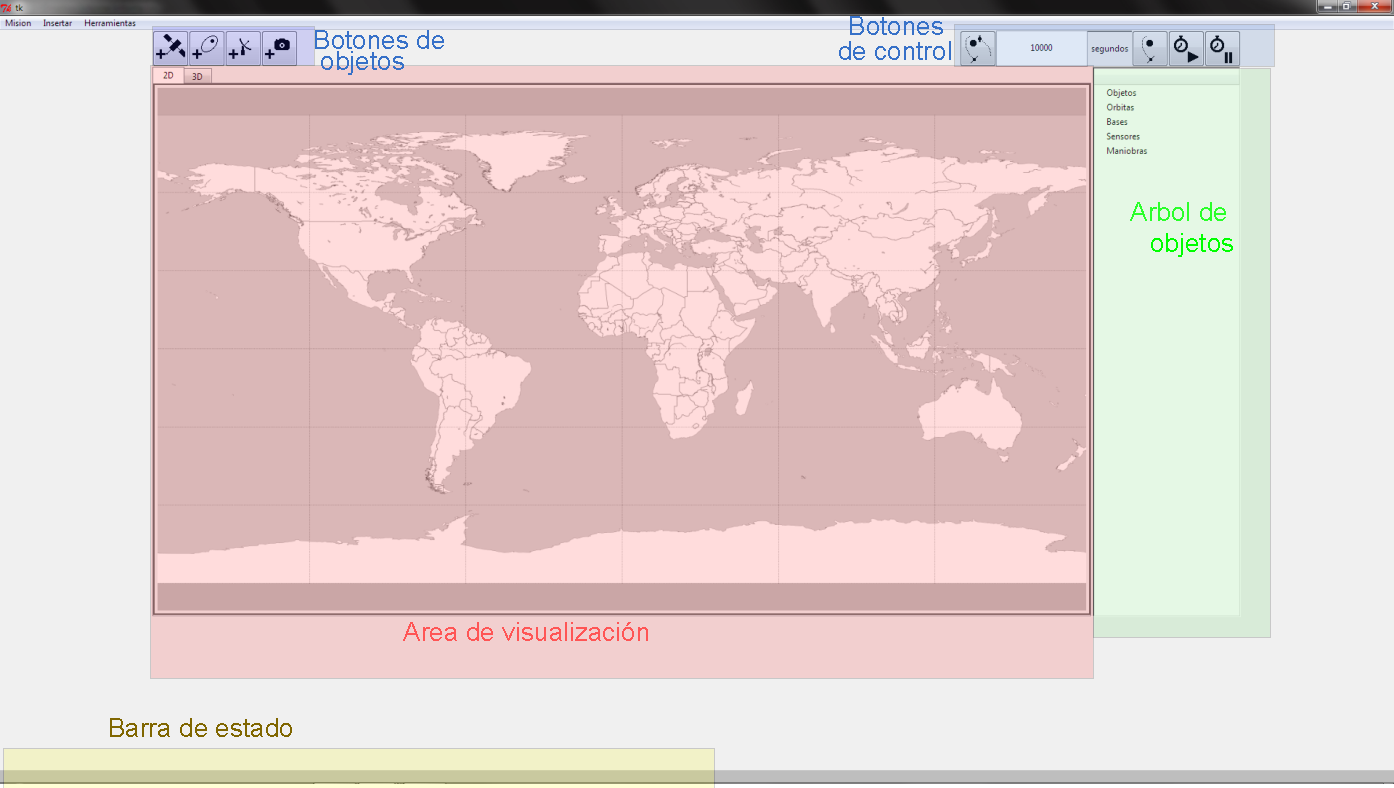
\includegraphics[scale=0.5]{interfazprincipal}
\par\end{centering}

\caption{Ventana principal}


\end{figure}


Una descripción de los distintos elementos puede encontrarse a continuación.


\subsubsection{Barra de estado}

Proporciona información sobre los distintos procesos que está llevando
a cabo el programa. Debido a la linealidad de algunas funciones del
código, resulta importante saber cuando ha acabado un proceso para
poder comenzar el siguiente. La barra de estado proporciona esta información
de manera sencilla, y puede dar una estimación del tiempo restante
para finalizar determinada tarea.


\subsubsection{Área de visualización}

Proporciona información visual de la posición de los elementos presentes
en la simulación. Las pestañas de la esquina superior izquierda permiten
alternar entre ver la representación en dos o tres dimensiones. Dentro
de la representación 3D las acciones
\begin{itemize}
\item Click izquierdo + arrastrar permite rotar la representación
\item Click derecho + arrastrar permite incrementar o disminuir el zoom
de la representación
\end{itemize}
permiten buscar una posición más favorable a la hora de visualizar
los datos.


\subsubsection{Botones de objetos}

Permiten introducir más elementos a la simulación, eligiendo el tipo
de objeto que se desea. Su función esta duplicada dentro del menu
\emph{Insertar} de la barra de herramientas superior para aumentar
la claridad.


\subsubsection{Arbol de objetos}

Permite conocer de un vistazo qué elementos están formando parte del
escenario, clasificados por tipo. Hacer click derecho sobre un elemento
abre un menú contextual sobre él que permite, entre otras cosas, borrarlo
del escenario, ocultarlo de las representaciones y abrir la ventana
de configuración del objeto.


\subsubsection{Botones de objetos}

Permiten controlar el flujo de integración de la simulación. Su función
específica se explicará más adelante


\subsubsection{Barra de herramientas}

Permite acceder a distintas funciones organizadas en menús temáticos.
El menú \emph{Misión} permite acceder a comandos relacionados con
el escenario en general. \emph{Nueva misión} permite cargar un escenario
vacío desde cero, mientras que \emph{Abrir} permite cargar uno preexistente.
\emph{Guardar }y \emph{Guardar como} permiten guardar el escenario
en su estado actual en un archivo para su uso posterior. Si es la
primera vez que se guarda el escenario actual, ambas funciones son
idénticas. Por último, \emph{Cerrar }hace que el programa se cierre,
perdiendo toda información no guardada.

El menú \emph{Insertar} cumple las mismas funciones que los distintos
botones de objetos, mientras que el menú \emph{Herramientas} permite
el acceso y uso de varias funciones extra.


\section{Organizando la simulación}

Ahora que ya se conocen las funciones básicas, vamos a organizar la
primera simulación con el programa. El orden en que se realicen los
pasos no es importante, siempre que se tenga en cuenta que la integración
numérica se llevará a cabo con los valores y objetos que se hayan
definido en el momento de lanzarla, por lo que cambiar parámetros
a mitad de simulación puede comprometer la validez y consistencia
de los resultados.


\subsection{Configurando los parámetros}

Hacer click en \emph{Parámetros}, dentro del menú \emph{Herramientas},
hace emerger una ventana que permite configurar el escenario y los
distintos parámetros que se van a usar. 
\begin{figure}


\begin{centering}
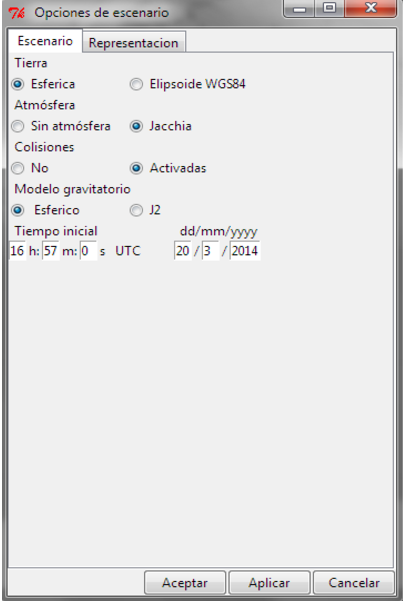
\includegraphics{parametros}
\par\end{centering}

\caption{Ventana de parámetros de escenario}
\end{figure}


\emph{Tierra }permite elegir entre una cálculo de tierra esférica
o el uso del elipsoide definido por el modelo WGS84

\emph{Atmósfera} permite incorporar a la simulación la perturbación
de la atmósfera, definida por el modelo Jacchia 77

\emph{Colisiones} permite desactivar el choque de los distintos objetos
contra la tierra, para realizar un estudio más teórico del problema

\emph{Modelo gravitatorio} alterna el uso de un modelo de gravedad
puramente esférico con la introducción de la perturbación J2 del EGM96

\emph{Tiempo inicial} permite elegir con detalle el instante en que
comenzará la simulación, parámetros que determinará las posiciones
relativas de la tierra y el sol a lo largo de la simulación

Puede observarse la existencia de otra pestaña llamada representación
que permite alterar varios valores conectados a la representación
gráfica del escenario. Tocar estos valores afecta únicamente a la
representación y nunca a la simulación numérica, pero relajarlos puede
suponer una mejora en el tiempo de cálculo del programa.


\subsection{Añadiendo elementos}

Ahora ya tenemos el escenario configurado a nuestro gusto, pero está
vacío. Es hora de añadir los elementos sobre los que tendrá lugar
la integración numérica. Los distintos objetos pueden añadirse desde
los botones presentes en la ventana principal o desde el menú \emph{Insertar,
}y el tipo seleccionado se puede cambiar dentro de la ventana de configuración
del objeto. Aunque las maniobras aparecen en el arbol, se crean de
manera distinta al resto de objetos desde otro menú, que ya se explicará
más adelante.


\subsubsection{Añadir satélites}

Al pulsar el botón con el símbolo del satélite o el elemento \emph{Añadir
sólido} del menú \emph{Insertar}, se crea una ventana que permite
la definición de un nuevo objeto de tipo sólido, la unidad básica
para la simulación. Es a los sólidos a los que se aplican las distintas
fuerzas y se hace la integración numérica.
\begin{figure}


\begin{centering}
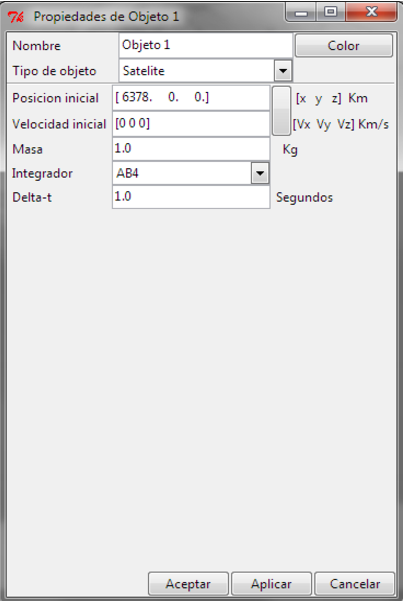
\includegraphics{satelite}
\par\end{centering}

\caption{Añadir sólido}


\end{figure}


Los campos \emph{Nombre }y\emph{ color} son puramente estéticos, y
permiten introducir el nombre con el que el programa se referirá al
objeto y el color con el que lo representará

Los campo de velocidad y posición iniciales permiten establecer las
condiciones iniciales del objeto, en el sistema de referencia ECI
(Earth Centered Inertial). Como estos campos pueden resultar confusos,
hacer click en el botón que aparece a su derecha lleva a otra ventana,
que permite configurar estos valores automáticamente a partir de una
órbita elíptica.

Los campos de \emph{Integrador} y \emph{Delta-t} permiten controlar
el proceso de integración numérica, pudiendo elegir entre Adams-Bashforth
de orden 4, Runge-Kutta 4 y predictor-corrector (AB4-AM4) 

Nótese que todos estos campos se aplican únicamente al objeto en particular,
por lo que es posible definir varios objetos iguales con distintos
integradores para comparar sus resultados, o modificar ligeramente
las condiciones iniciales para ver como se propaga esa perturbación.


\subsubsection{Añadir órbitas}

Al presionar el botón correspondiente se abre la ventana de configuración
de la órbita, que permite configurarla a partir de sus elementos clásicos.
Las órbitas se usan como elementos auxiliares para definir otros objetos
o para calcular distintas maniobras entre ellas

\begin{figure}


\begin{centering}
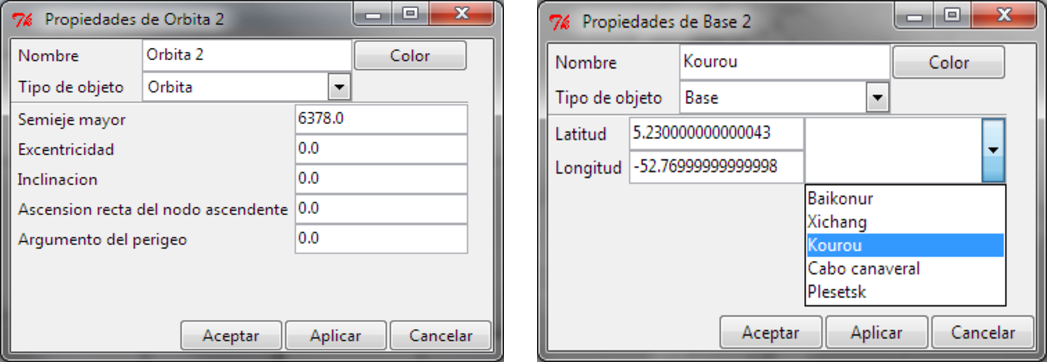
\includegraphics[scale=0.75]{orbitabase}
\par\end{centering}

\caption{Añadir órbitas y bases}


\end{figure}



\subsubsection{Añadir bases}

De la misma manera que el resto de objetos, permite congiurar el nombre
y el color con el que se representará. La posición de la base viene
dada por sus coordenaas geográficas, que se pueden introducir a mano
o seleccionar de una pequeña lista que se despliega al hacer click
en el pequeño menú de la derecha.


\subsubsection{Añadir sensores}

Similarmente, al añadir un sensor se pueden configurar varios de sus
valores.

\begin{figure}


\begin{centering}
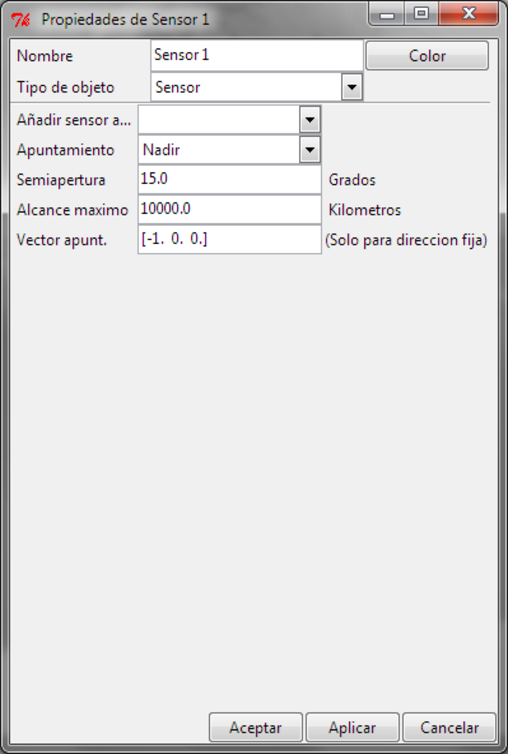
\includegraphics{sensor}
\par\end{centering}

\caption{Añadir sensor}


\end{figure}


Los sensores so objetos un poco especiales, ya que no tienen posición
fija, sino que se añaden a otro objeto de tipo sólido o de tipo base.
Adquirirán su posición a partir de la de su objeto padre y calcularán
sus datos a partir de ella.

El apuntamiento de un sensor es fundamental a la hora de calcular
sus actuaciones, por lo que el programa deja elegir entre un apuntamiento
fijo a nadir, el punto subsatélite del satélite, un apuntamiento a
cenit, la dirección contraria, y apuntamiento a una dirección fija.
Está dirección es un vector del sistema ECI, y puede definirse a través
de la entrada del vector de apuntamiento.

El sensor se modela como cónico por simplicidad, y los valores de
semiapertura y de alcance máximo son configurables.


\subsection{Controlando la simulación}

El control de la simulación se hace mediante los botones de control
de la ventana principal
\begin{figure}
\begin{centering}
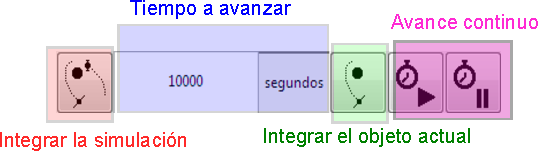
\includegraphics{control}
\par\end{centering}

\caption{Control de la simulación}


\end{figure}


La simulación puede avanzar un tiempo determinado o hacerse de manera
continua e indefinida. Esta elección se hace mediante el bloque de
control de la esquina superior derecha de la pantalla principal. 


\subsubsection{Avance fijo}

El avance fijo es la opción que permite un mayor control del escenario,
permitiendo elegir con exactitud cuanto tiempo se quiere integrar.
El valor predefinido son 10000 segundos, pero haciendo click sobre
el número se puede cambiar al valor deseado. 

El primer botón de la izquierda permite integrar todo el escenario.
Está acción lanzará la integración de todos los elementos presentes
en el escenario a la vez a lo largo del tiempo deseado. El progreso
de cada objeto por separado se muestra en la barra de estado inferior,
y al terminar la integración se mostrarán las trazas y trayectorias
de todos los elementos presentes.

El segundo botón, a la derecha del tiempo a avanzar, permite integrar
un único objeto cada vez. Cada objeto lleva una cuenta por separado
del tiempo transcurrido desde el instante inicial, por lo que es posible
manejar cada objeto por separado con un tiempo de integración diferente.
El objeto que se va a integrar puede verse en el árbol de objetos,
ya que el objeto actual tendrá un pequeño símbolo delante de su nombre.
Para cambiar el objeto que se va a integrar, basta con hacer doble
click sobre el elemento deseado en el arbol
\begin{figure}
\begin{centering}
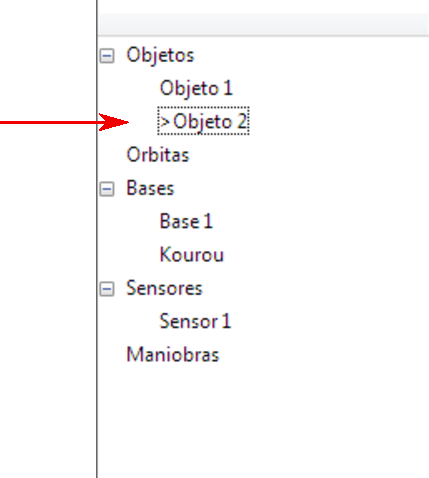
\includegraphics{arbol}
\par\end{centering}

\caption{Arbol y objeto seleccionado}


\end{figure}



\subsubsection{Avance continuo}

En lugar de integrar una cantidad fija de tiempo, puede quererse ver
la evolución del escenario de manera continua. Los dos últimos botones
permiten este control, iniciando y pausando este proceso. Se hace
una cortaq integración seguida de la representación de los datos obtenidos,
repitiéndose el proceso hasta que el usuario lo pause. Téngase en
cuenta que el dibujado de datos es un proceso lento en el programa,
por lo que el rendimiento puede verse comprometido, por lo que puede
resultar conveniente reducir la carga gráfica dentro de los parámetros
del programa para acelerar este proceso.


\section{Resultados}

Ahora que ya hemos introducido los elementos que queriamos analizar,
y hemos integrado hasta el punto necesario, vamos a ver como acceder
a los resultados.


\subsection{Representación gráfica}

El más evidente se proporciona sobre las representaciones 2D y 3D.
Las trayectorias de los distintos objetos y las trazas que dejan sobre
el mapa. Esta información, cualitativa de momento, resulta muy útil
para un ingeniero con experiencia en mecánica orbital, ya que permite
estimar fácilmente parámetros esenciales como la cobertura, la repetitividad
de las trazas, forma de las órbitas, etc.

\begin{figure}
\begin{centering}
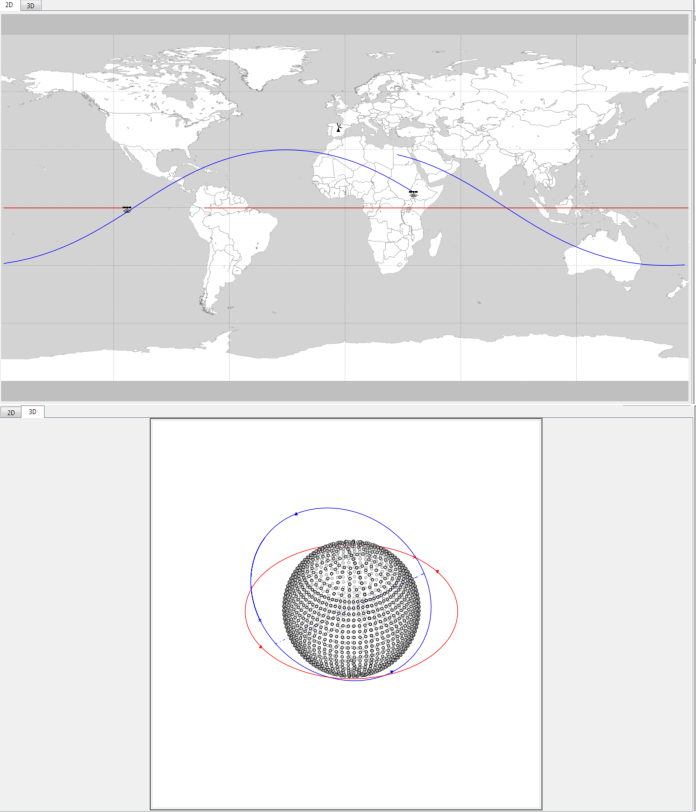
\includegraphics{representacion}
\par\end{centering}

\caption{Representaciones bidimensional y tridimensional}


\end{figure}


Sobre el mapa se representan también las posiciones actuales de los
distintos objetos mediante unos pequeños iconos. Sobre la representación
tridimensional, se marcan la linea de nodos y las posiciones del satélite,
del apogeo y del perigeo para facilitar la lectura.

Los objetos tipo órbita únicamente son representados en tres dimensiones
y, si hay presente algún sensor, se representa además el cono de visibilidad
sobre el gráfico tridimensional y la zona de cobertura sobre el mapa.
\begin{figure}
\begin{centering}
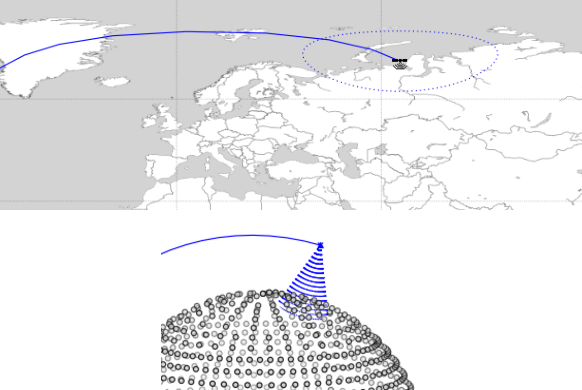
\includegraphics{repsensor}
\par\end{centering}

\caption{Representación del sensor}


\end{figure}



\subsection{Acceso a datos instantáneos}

A través del árbol de objetos se puede acceder a determinada información
del estado actual del objeto. Haciendo click derecho, se despliega
un menú contextual, uno de cuyos elementos se llama \emph{Información}.
Al pulsar sobre él, se abre una ventana que proporciona algunos datos
, los fundamentales para cada tipo de objeto, que pueden resultar
útiles
\begin{figure}


\begin{centering}
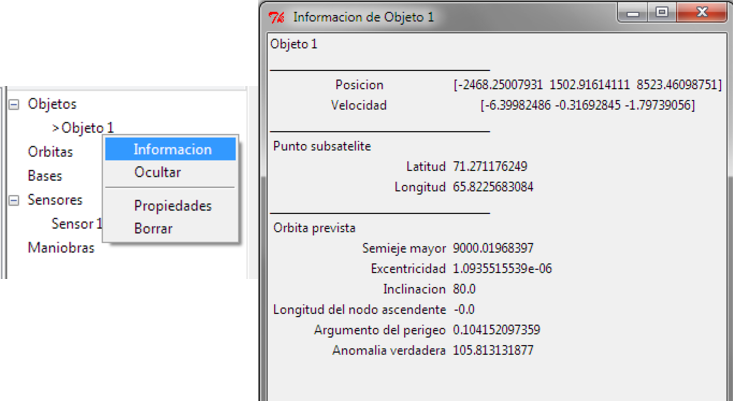
\includegraphics{informacion}
\par\end{centering}

\caption{Ventana de información}


\end{figure}



\subsection{Acceso a todos los datos}

Dentro del menú \emph{Herramientas}, el elemento \emph{Resultados}
permite conocer una gran cantidad de datos de la simulación.

\begin{figure}


\begin{centering}
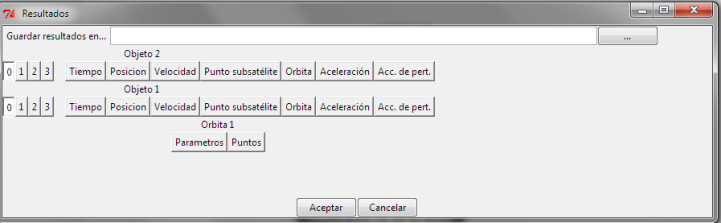
\includegraphics{resultados}
\par\end{centering}

\caption{Ventana de resultados}


\end{figure}


Aparecen los objetos presentes en la simulación, y una serie de opciones
dependientes del tipo de objeto. En la parte superior, debe introducirse
la ruta de un archivo de texto, archivo al que se volcarán los resultados.
Puede introducirse directamente o usar para ello el botón presente
en la parte derecha, que abrirá un diálogo de explorador para seleccionar
el archivo.

Debajo de cada objeto se presentan las distintas posibilidades específicas.
Haciendo click sobre cada uno de los botones se puede selecciona ese
dato para volcarlo en el archivo, con un formato adecuado, o ignorarlo,
si no interesa conocerlo en el escenario actual.

Los objetos tipo sólido tienen además cuatro botones adicionales,
los 4 primeros, que no corresponden a ningún dato, sino a la frecuencia
del resto. Así, se puede seleccionar si se quieren conocer los datos
cada 1 punto ($10^{0}$), 10 ($10^{1}$), 100 ($10{}^{2}$) o 1000
($10{}^{3}$), de manera que la cantidad de información a procesar
después sea menor.

Al hacer click en el botón aceptar, se creará (o reemplazará) el archivo
deseado con los datos seleccionados.


\section{Herramientas}

El programa dispone además de algunas herramientas útiles a la hora
de analizar la misión de un satélite. Deben usarse después de haber
introducido los elementos necesarios y haber integrado el escenario
hasta el punto deseado, accediendo a ellas a través del menú \emph{Herramientas}.


\subsection{Asistente de visibilidad}

Sirve para comprobar si un objeto ve a otro a lo largo de su trayectoria.
Una vez que se tienen las trayectorias deseadas calculadas, accediendo
a esta herramienta abre una nueva ventana que hará de menú.

\begin{figure}


\begin{centering}
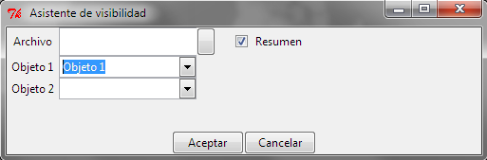
\includegraphics{visibilidad}
\par\end{centering}

\caption{Ventana de visibilidad}


\end{figure}


Dentro de esta ventana debe elegirse un archivo de manera parecida
a la ventana de resultados: Introduciendo la ruta directamente o pulsando
el botón de la derecha.

Los dos campos inferiores permiten elegir los dos objetos que se quieren
analizar de entre los presentes en el escenario. Pueden ser sólidos,
bases o sensores debidamente definidos e integrados. En el segundo
objeto puede elegirse además el sol, que permitirá calcular el tiempo
en que un objeto está iluminado para, por ejemplo, calcular los eclipses
de un satélite o los amaneceres de una posición geográfica.

La pequeña opción de resumen está activada por defecto. Si se desactiva,
vuelca al archivo elegido información detallada de las posiciones
de los dos objetos en cada instante y calcula si se ven entre ellos
o no. Si se deja activada, vuelca únicamente los periodos en que se
ven, marcando entrada, salida y duración de cada periodo.

Al hacer click en el botón aceptar, se lanza el análisis, calculando
las posiciones de los dos objetos y comprobando después si la linea
de visión está obstruida por la tierra. Si uno de los dos objetos
es un sensor, comprueba además que la linea de visión este dentro
del cono de cobertura. Las posiciones se calculan en instantes enteros
cada segundo y si las posiciones de los objetos no coinciden con este
instante, se interpolan linealmente entre los dos más próximos.


\subsection{Asistente de maniobras}

Otra herramienta muy útil para el análisis de misión es el cálculo
de las distintas maniobras que tendrá que hacer el satélite. Tanto
para definir la misión como para dimensionar la masa de combustible
y el motor, resulta fundamental conocer desde el comienzo los impulsos
que habrá que realizar a lo largo de la vida del satélite. Para ello,
el programa cuenta con una herramienta para facilitar el cálculo de
estos elementos.

\begin{figure}


\begin{centering}
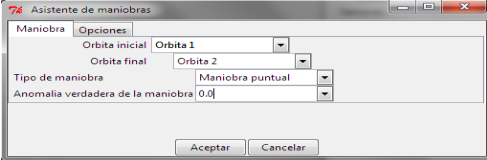
\includegraphics{maniobras}
\par\end{centering}

\caption{Ventana de maniobras}


\end{figure}


Se abre un diálogo que permite seleccionar dos órbitas de entre las
presentes en el escenario. Al hacer click en maniobra puntual, el
programa calcula las intersecciones de los dos objetos y permite elegir
el punto donde se quiere calcular la maniobra, en forma de la anomalía
verdadera de la órbita inicial. Una vez se han seleccionado todos
los parámetros necesarios, hacer click en el botón aceptar calculará
la maniobra, desplegando una ventana con información sobre ella y,
si se ha seleccionado así, añadiendo el objeto al escenario para que
pueda revisarse a posteriori.
\begin{figure}


\begin{centering}
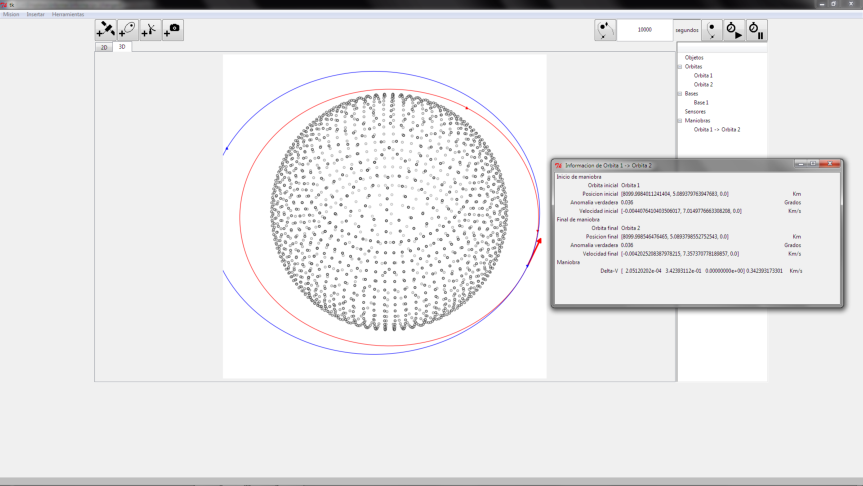
\includegraphics[scale=0.8]{maniobrasresultados}
\par\end{centering}

\caption{Resultados de la maniobra}


\end{figure}



\chapter{Validación}

En este capítulo va a tratarse la verificación y validación de todos
los elementos implicados en la simulación y de su conjunto, abordando
una de las partes más importantes de la construcción de todo simulador.


\section{Objetivo}

Una vez se ha construido un simulador, se espera tener una serie de
datos, normalmente numéricos, que sean la respuesta del sistema simulado
a una serie de entradas. Sin embargo, la validez de estos datos está
todavía en entredicho. No se pueden, o no se deben, usar esta salida
de datos sin comprobar antes si se acercan o se alejan de la realidad.

Como normalmente se hace una simulación para obtener la solución a
un sistema para el que no se tiene respuesta, resulta difícil comparar
nuestra solución directamente con la realidad y hay que buscar otra
estrategia. 

Una posible solución es usar varios simuladores independientes, introducir
el mismo problema y comprar los resultados entre las soluciones que
aporta cada uno de ellos, confiando en que en la multitud esté la
respuesta correcta. Este proceso, aunque beneficioso, es largo y costoso,
por lo que debe reducirse en la medida de lo posible.

La otra ruta más común consiste en elegir un problema para el que
sí se tenga la solución. Se compara la simulación con ella y se extrapola
la validez del sistema hasta otros problemas. Esta es la vía más rápida,
pero no siempre se tiene acceso a una solución de un problema lo suficientemente
complejo como para resultar útil en este proceso.

El proceso de validación, se elija la ruta que se elija, consistirá
en comparar la solución numérica con una solución patrón, viendo cuanto
se desvía y comprobando que este error está dentro de las tolerancias
del proyecto.

Se puede hablar también de un proceso de validación del software,
comprobando que cumple los requisitos y objetivos que se le habían
planteado al inicio del proyecto, y evaluando el programa desde el
punto de vista del usuario final.


\section{Métodos de validación}

Se plantean cuatro posibles métodos para realizar la validación de
este programa.
\begin{enumerate}
\item Verificación del código. La manera más sencilla, rápida e intuitiva
de comprobar que el simulador ha implementado correctamente los modelos
definidos es, efectivamente, comprobar directamente que los modelos
se han implementado bien. Este proceso se hace conociendo los modelos
teóricos que se han implementado y navegando el código para inspeccionarlo
y comprobar que la lógica y estructura del programa corresponde con
la del modelo teórico. Este proceso no es ni mucho menos suficiente
para asegurar la validez de la simulación, pero desde luego es necesario
para abordar futuros pasos. El autor del programa ya ha realizado
numerosas veces este método, pero se invita a que el lector haga una
lectura crítica y compruebe por si mismo las funciones del simulador.
Para ello, se ha intentado diseñar el código de manera clara y simple,
con funciones modulares autodescriptivas y autocontenidas, de manera
que su inspección resulte fácil. Como el programa se distribuye con
su código abierto, ayudado por las ecuaciones presentadas en el capítulo
3 cualquiera puede realizar esta tarea.
\item Validación del código frente a la solución analítica. Si el problema
tiene una solución analítica sencilla y conocida, resulta muy fácil
comparar los resultados numéricos obtenidos en el simulador con esta
solución. Sin embargo, el rango de problemas que cumplen estos requirimientos
es alarmantemente bajo, por lo que su aplicación a la validación de
este programa no es posible más que en los procesos más sencillos.
\item Validación del código frente a la solución obtenida en otro simulador.
Si otro programa resuelve la misma gama de problemas y ya tiene sus
soluciones verificadas y validadas, resulta relativamente fácil comprobar
la similitud entre las dos soluciones y extrapolarla a la similitud
con la realidad. Elegir con criterio el programa que se va a usar
como patrón resulta fundamental, y resulta conveniente elegir paquetes
de software robustos, con muchos kilómetros encima y cuyo uso esté
extendido en la industria. En este proyecto va a usarse como fuente
de comparaciones el software STK en su versión 10, distribuido por
Analytical Graphics, Inc. %
\footnote{www.agi.com/products/stk%
}(AGI), un programa con mucho historial de servicio en la industria
y prestaciones más que probadas.
\item Validación de la solución frente a datos reales. Qué mejor manera
de estimar cuanto se acerca nuestra solución a la realidad que ver
cuanto se acerca nuestra solución a la realidad. Aunque este método
pueda resultar el más adecuado, no siempre es fácil obtener datos
de una misión real y, cuando se tienen, no resulta nada fácil discriminar
los efectos que se quieren verificar del resto de efectos y del ruido.
\end{enumerate}
Naturalmente, todas las pruebas que se van a realizar son reproducibles
por el usuario y se invita al lector a que someta al programa a todos
aquellos procesos que considere adecuados.


\section{Validación del estado inicial}

Antes de ver como se comporta la integración numérica del programa,
vamos a comprobar que todos los elementos y sistemas de referencia
están bien definidos, y que las conversiones entre ellos funcionan
correctamente.

La NASA publica con regularidad los datos de la órbita que sigue la
estación espacial internacional, además de su posición en distintos
sistemas de referencia. Vamos a usarlos para comprobar que nuestro
ECI está bien definido.

\bigskip{}


\noindent\makebox[\textwidth]{%

\begin{tabular*}{19cm}{@{\extracolsep{\fill}}|c||c||c||c||c||c|}
\hline 
\multicolumn{3}{|c||}{Órbita ISS J2000} & \multicolumn{3}{c|}{NASA}\tabularnewline
\hline 
\hline 
\multicolumn{6}{|c|}{23/1/2015 12:00:00}\tabularnewline
\hline 
\hline 
Semieje mayor  & Excentricidad & Inclinación & Longitud nodo asc & Argumento perigeo & Anomalia verdadera\tabularnewline
\hline 
\hline 
6789.96481 Km & 0.0011196 & 51.746º & 86.254º & 37.759º & 339.336º\tabularnewline
\hline 
\end{tabular*}

}\bigskip{}


Introduciendo estos datos en el programa, se obtiene

\bigskip{}


\noindent\makebox[\textwidth]{%

\begin{tabular}{|c|cc|c|c|c|c|}
\hline 
\multicolumn{7}{|c}{Posición ISS J2000}\tabularnewline
\hline 
 & \multicolumn{2}{c|}{Simulador} & \multicolumn{2}{c|}{NASA} & \multicolumn{2}{c|}{STK}\tabularnewline
\hline 
\multirow{3}{*}{Posición Km} & \multicolumn{2}{c|}{-808.29378} & \multicolumn{2}{c|}{-808.30168} & \multicolumn{2}{c|}{-808.300178}\tabularnewline
 & \multicolumn{2}{c|}{6549.97816383} & \multicolumn{2}{c|}{6549.98438} & \multicolumn{2}{c|}{6549.984541}\tabularnewline
 & \multicolumn{2}{c|}{1565.73046259} & \multicolumn{2}{c|}{1565.70111} & \multicolumn{2}{c|}{1565.700474}\tabularnewline
\hline 
\multirow{3}{*}{Velocidad Km/s} & \multicolumn{2}{c|}{-4.6762487} & \multicolumn{2}{c|}{-4.67623009} & \multicolumn{2}{c|}{-4.676235}\tabularnewline
 & \multicolumn{2}{c|}{-1.95617957} & \multicolumn{2}{c|}{-1.956160859} & \multicolumn{2}{c|}{-1.956159}\tabularnewline
 & \multicolumn{2}{c|}{5.75617466} & \multicolumn{2}{c|}{5.756198415} & \multicolumn{2}{c|}{5.756193}\tabularnewline
\hline 
Módulo error pos / \% contra módulo &  &  & 0.0310262 & 0.00045\% & 0.0313196 & 0.00046\%\tabularnewline
\cline{1-1} \cline{4-7} 
Módulo error vel / \% contra módulo &  &  & 3.55135$\cdot10^{-5}$ & 0.00046\% & 3.07761$\cdot10^{-5}$ & 0.00040\%\tabularnewline
\cline{1-1} \cline{4-7} 
\end{tabular}

}\bigskip{}


La posición de este punto sobre la tierra en el instante señalado
es

\bigskip{}


\begin{tabular}{|c|c|c|}
\hline 
\multicolumn{3}{|c}{Traza ISS}\tabularnewline
\hline 
\hline 
 & Simulador & STK\tabularnewline
\hline 
Latitud & 13.427183591 & 13.414\tabularnewline
\hline 
Longitud & 154.674416216 & 154.741\tabularnewline
\hline 
Error latitud &  & 0.013183591\tabularnewline
\cline{1-1} \cline{3-3} 
Error longitud &  & 0.066583784\tabularnewline
\cline{1-1} \cline{3-3} 
Distancia error sobre la tierra &  & 7.349 Km\tabularnewline
\cline{1-1} \cline{3-3} 
\end{tabular}

\bigskip{}



\section{Validación de la integración a corto plazo}

Una vez que se ha comprobado que el sistema de cálculo de órbitas
y los distintos sistemas de referencia funcionan correctamente, vamos
a ver cómo se comporta la integración numérica del simulador. Para
ello se sigue el mismo procedimiento, se elige una órbita (La de la
ISS) y se integra en el tiempo la misma cantidad mediante el simulador
y el STK para hallar el punto final y calcular sus diferencias. Además
al hacerse estos primeros test sin perturbaciones, va a calcularse
también la solución analítica que proporcionan las ecuaciones de mecánica
orbital.

\bigskip{}


\begin{tabular}{|c|c|c|c|}
\hline 
\multicolumn{4}{|c}{Posición ISS J2000}\tabularnewline
\hline 
\multicolumn{2}{|c|}{Integrador: Adams-Bashforth 4} & \multicolumn{2}{c|}{Paso de integración: 1. segundo}\tabularnewline
\hline 
\multicolumn{2}{|c|}{Tiempo de integración: 90 minutos} & \multicolumn{2}{c|}{Perturbaciones: Ninguna}\tabularnewline
\hline 
\hline 
 & Simulador & STK & Analítica\tabularnewline
\hline 
\multirow{3}{*}{Posición Km} & -11.872329 & -12.082321 & -11.89909952\tabularnewline
 & 6759.06956 & 6759.032671 & 6759.049063\tabularnewline
 & 575.10382 & 575.322834 & 575.1360026\tabularnewline
\hline 
\multirow{3}{*}{Velocidad Km/s} & -4.764617 & -4.764604 & -4.764616\tabularnewline
 & -0.522276 & -0.522615 & -0.5223207\tabularnewline
 & 5.986831 & 5.986813 & 5.9868277\tabularnewline
\hline 
\hline 
Módulo error pos &  & 0.3056543 & 0.04661\tabularnewline
\cline{1-1} \cline{3-4} 
Módulo error vel &  & 0.000339 & 4.48328$\cdot10^{-5}$\tabularnewline
\cline{1-1} \cline{3-4} 
\end{tabular}\bigskip{}


\begin{tabular}{|c|c|c|c|}
\hline 
\multicolumn{4}{|c}{Posición ISS J2000}\tabularnewline
\hline 
\multicolumn{2}{|c|}{Integrador: Runge-Kutta 4} & \multicolumn{2}{c|}{Paso de integración: 1. segundo}\tabularnewline
\hline 
\multicolumn{2}{|c|}{Tiempo de integración: 90 minutos} & \multicolumn{2}{c|}{Perturbaciones: Ninguna}\tabularnewline
\hline 
\hline 
 & Simulador & STK & Analítica\tabularnewline
\hline 
\multirow{3}{*}{Posición Km} & 120.219219 & -12.082321 & -11.89909952\tabularnewline
 & 6817.208853 & 6759.032671 & 6759.049063\tabularnewline
 & 412.746093 & 575.322834 & 575.1360026\tabularnewline
\hline 
\multirow{3}{*}{Velocidad Km/s} & -4.745979 & -4.764604 & -4.764616\tabularnewline
 & -0.283243 & -0.522615 & -0.5223207\tabularnewline
 & 5.983051 & 5.986813 & 5.9868277\tabularnewline
\hline 
\hline 
Módulo error pos &  & 217.5301 & 217.2747\tabularnewline
\cline{1-1} \cline{3-4} 
Módulo error vel &  & 0.2401249 & 0.239832\tabularnewline
\cline{1-1} \cline{3-4} 
\end{tabular}\bigskip{}


\begin{tabular}{|c|c|c|c|}
\hline 
\multicolumn{4}{|c}{Posición ISS J2000}\tabularnewline
\hline 
\multicolumn{2}{|c|}{Integrador: Predictor-Corrector} & \multicolumn{2}{c|}{Paso de integración: 1. segundo}\tabularnewline
\hline 
\multicolumn{2}{|c|}{Tiempo de integración: 90 minutos} & \multicolumn{2}{c|}{Perturbaciones: Ninguna}\tabularnewline
\hline 
\hline 
 & Simulador & STK & Analítica\tabularnewline
\hline 
\multirow{3}{*}{Posición Km} & 146.599039 & -12.082321 & -11.89909952\tabularnewline
 & 6828.529375 & 6759.032671 & 6759.049063\tabularnewline
 & 380.297794 & 575.322834 & 575.1360026\tabularnewline
\hline 
\multirow{3}{*}{Velocidad Km/s} & -4.741370 & -4.764604 & -4.764616\tabularnewline
 & -0.236034 & -0.522615 & -0.5223207\tabularnewline
 & 5.981129 & 5.986813 & 5.9868277\tabularnewline
\hline 
\hline 
Módulo error pos &  & 260.853 & 260.597584\tabularnewline
\cline{1-1} \cline{3-4} 
Módulo error vel &  & 0.287577 & 0.287285\tabularnewline
\cline{1-1} \cline{3-4} 
\end{tabular}

\bigskip{}


Puede comprobarse que el integrador que mejor se comporta es el Adams-Bashforth
de cuarto orden, alcanzando con él una gran precisión.

Puede surgir la duda de cómo cambia el comportamiento frente a distintos
pasos de integración. Se repiten las pruebas, usando el integrador
Adams-Bashforth y variando el $\triangle t$

\bigskip{}


\begin{tabular}{|c|c|c|c|c|}
\hline 
$\triangle t$ & Posición Km & Velocidad Km/s & Error pos con STK & Error vel con STK\tabularnewline
\hline 
\multirow{3}{*}{0.1} & 1044.1713 & -4.5612 & \multirow{3}{*}{1700.18} & \multirow{3}{*}{1.872172}\tabularnewline
 & 6853.5761 & 1.3356 &  & \tabularnewline
 & -753.5961 & 5.8834 &  & \tabularnewline
\hline 
\multirow{3}{*}{0.5} & -12.023336 & -4.764616 & \multirow{3}{*}{0.06672655} & \multirow{3}{*}{6.9231$\cdot10^{-5}$}\tabularnewline
 & 6759.039837 & -0.522547 &  & \tabularnewline
 & 575.292472 & 5.986808 &  & \tabularnewline
\hline 
\multirow{3}{*}{1.0} & -11.872329 & -4.764617 & \multirow{3}{*}{0.3056543} & \multirow{3}{*}{3.3972$\cdot10^{-4}$}\tabularnewline
 & 6759.06956 & -0.522276 &  & \tabularnewline
 & 575.10382 & 5.986831 &  & \tabularnewline
\hline 
\multirow{3}{*}{1.5} & -11.620536 & -4.764617 & \multirow{3}{*}{0.710934} & \multirow{3}{*}{7.93$\cdot10^{-4}$}\tabularnewline
 & 6759.119175 & -0.521824 &  & \tabularnewline
 & 574.789261 & 5.986869 &  & \tabularnewline
\hline 
\multirow{3}{*}{2.0} & -11.268124 & -4.764618 & \multirow{3}{*}{1.27889} & \multirow{3}{*}{1.42$\cdot10^{-3}$}\tabularnewline
 & 6759.188559 & -0.521193 &  & \tabularnewline
 & 574.348998 & 5.986923 &  & \tabularnewline
\hline 
\multirow{3}{*}{5.0} & -7.0404 & -4.7646 & \multirow{3}{*}{8.0948} & \multirow{3}{*}{9.02$\cdot10^{-3}$}\tabularnewline
 & 6760.0180 & -0.513617 &  & \tabularnewline
 & 569.0671 & 5.9875 &  & \tabularnewline
\hline 
\multirow{3}{*}{10.0} & 8.0503 & -4.7645 & \multirow{3}{*}{32.422} & \multirow{3}{*}{0.0361}\tabularnewline
 & 6762.9297 & -0.4866 &  & \tabularnewline
 & 550.2094 & 5.9897 &  & \tabularnewline
\hline 
\end{tabular}

\bigskip{}


Puede comprobarse que el mejor resultado se consigue usando pasos
de tiempo menores que 1. Sin embargo, esto aumenta significativamente
el tiempo requerido de computación y alarga el proceso. Usar pasos
muy pequeños, además de disparar el tiempo requerido para hacer la
integración, introducen mucho error de redondeo y dan lugar a resultados
malos. Usando pasos mayores que 1 se consigue reducir el tiempo de
integración manteniendo todavía una buena precisión en los cálculos,
por lo que para grandes integraciones puede resultar una estrategia
rentable. Eligiendo usar un paso de tiempo de 1, se alcanza un compromiso
adecuado entre precisión y tiempo de cálculo.


\section{Validación de la integración a largo plazo}

Que el proceso de integración sea preciso a corto plazo no quiere
decir que lo sea a largo. El problema de mecánica orbital es inestable
en el sentido de \emph{Lyapunov}: Perturbaciones en el estado inicial,
por pequeñas que sean, se propagan irremediablemente en el tiempo
hasta hacerse tan grandes como queramos. Esto hace que la integración
a muy largo plazo sea inviable sin implementar ciertas técnicas y
trucos que regularicen los resultados en cada paso. 

Vamos a integrar el mismo problema, pero esta vez durante 10 dias,
y comprobar como ha evolucionado la precisión.

\bigskip{}


\begin{tabular}{|c|c|c|c|}
\hline 
\multicolumn{4}{|c}{Posición ISS J2000}\tabularnewline
\hline 
\multicolumn{2}{|c|}{Integrador: Adams-Bashforth 4} & \multicolumn{2}{c|}{Paso de integración: 1. segundo}\tabularnewline
\hline 
\multicolumn{2}{|c|}{Tiempo de integración: 10 dias} & \multicolumn{2}{c|}{Perturbaciones: Ninguna}\tabularnewline
\hline 
\hline 
 & Simulador & STK & Analítica\tabularnewline
\hline 
\multirow{3}{*}{Posición Km} & -11.872329 & -12.082321 & -11.89909952\tabularnewline
 & 6759.06956 & 6759.032671 & 6759.049063\tabularnewline
 & 575.10382 & 575.322834 & 575.1360026\tabularnewline
\hline 
\multirow{3}{*}{Velocidad Km/s} & -4.764617 & -4.764604 & -4.764616\tabularnewline
 & -0.522276 & -0.522615 & -0.5223207\tabularnewline
 & 5.986831 & 5.986813 & 5.9868277\tabularnewline
\hline 
\hline 
Módulo error pos &  & 0.3056543 & 0.04661\tabularnewline
\cline{1-1} \cline{3-4} 
Módulo error vel &  & 0.000339 & 4.48328$\cdot10^{-5}$\tabularnewline
\cline{1-1} \cline{3-4} 
\end{tabular}\bigskip{}


\appendix

\chapter{Datos de validación}


\section{Datos NASA}


\subsection{Posición ISS inicial}

\noindent\resizebox{\textwidth}{!}{%

\begin{lstlisting}
  ISS  TRAJECTORY DATA
 
   Lift off time (UTC)  :  N/A
   Area (sq ft)  :  17222.26
   Drag Coefficient (Cd)  :   2.00
   Monthly MSFC 50% solar flux (F10.7-jansky)  :   132.9
   Monthly MSFC 50% earth geomagnetic index (Kp)  :   2.186
   ET - UTC  (sec) :   67.18
   UT1 - UTC (sec) :    0.00
 
 
   Maneuvers contained within the current ephemeris are as follows:
 
 
   IMPULSIVE TIG (GMT)   M50 DVx(FPS)      LVLH DVx(FPS)      DVmag(FPS) 
   IMPULSIVE TIG (MET)   M50 DVy(FPS)      LVLH DVy(FPS)      Invar Sph HA
   DT                    M50 DVz(FPS)      LVLH DVz(FPS)      Invar Sph HP 
   ------------------------------------------------------------------------
   028/18:42:08.283           1.2              -1.9              1.9    
   N/A                        0.9               0.3              220.3  
   000/00:04:12.566          -1.2              -0.0              216.7  
   
 
 
    Coasting Arc #1 (Orbit 552)
    ---------------------------------------
 
    Vector Time (GMT): 2015/023/12:00:00.000
    Vector Time (MET): N/A
    Weight (LBS)     : 950073.3
 
              M50 Cartesian                         M50 Keplerian  
    -----------------------------------       --------------------------------
     X    =        -727392.70                 A    =         6789964.81  meter
     Y    =        6558570.91  meter          E    =           .0011196
     Z    =        1569431.26                 I    =           52.02376
     XDOT =      -4669.795875                 Wp   =           37.73357
     YDOT =      -1903.904340  meter/sec      RA   =           85.62907  deg
     ZDOT =       5778.898520                 TA   =          339.33603
                                              MA   =          339.38127
                                              Ha   =            220.652  n.mi
                                              Hp   =            217.689
 
              M50 Cartesian                         J2K Cartesian  
    -----------------------------------       --------------------------------
     X    =       -2386458.99                 X    =         -808301.68
     Y    =       21517621.08  feet           Y    =         6549984.38  meter
     Z    =        5149052.70                 Z    =         1565701.11
     XDOT =     -15320.852608                 XDOT =       -4676.230090
     YDOT =      -6246.405316  feet/sec       YDOT =       -1956.160859  meter/sec
     ZDOT =      18959.640815                 ZDOT =        5756.198415
 
              TDR Cartesian                         TDR Cartesian  
    -----------------------------------       --------------------------------
     X    =      -19583286.76                 X    =        -5968985.80
     Y    =        9239834.20  feet           Y    =         2816301.46  meter
     Z    =        5131889.62                 Z    =         1564199.96
     XDOT =      -2119.045564                 XDOT =        -645.885088
     YDOT =     -14991.702956  feet/sec       YDOT =       -4569.471061  meter/sec
     ZDOT =      18862.830949                 ZDOT =        5749.390873
  
  
    The mean element set is posted at the UTC for which position is
    just north of the next ascending node relative to the above
    vector time
 
 
    TWO LINE MEAN ELEMENT SET
  
    ISS
    1 25544U 98067A   15023.56127426  .00016717  00000-0  10270-3 0  9001
    2 25544  51.6451  86.1253 0006010 294.3336  65.7188 15.53554402  5538
  
  
    Satellite: ISS
    Catalog Number: 25544
    Epoch time:      15023.56127426   =   yrday.fracday
    Element set:     900
    Inclination:       51.6451  deg
    RA of node:        86.1253  deg
    Eccentricity:     .0006010     
    Arg of perigee:   294.3336  deg
    Mean anomaly:      65.7188  deg
    Mean motion:   15.53554402  rev/day
    Decay rate:    1.67170E-04  rev/day^2
    Epoch rev:             553
    Checksum:              283
\end{lstlisting}


}


\section{Datos STK}

\noindent\resizebox{\textwidth}{!}{%

\begin{lstlisting}
                                                                                                 27 Jan 2015 18:09:31
Satellite-Satellite1:  J2000 Position & Velocity


       Time (UTCG)             x (km)          y (km)          z (km)       vx (km/sec)    vy (km/sec)    vz (km/sec)
------------------------    ------------    ------------    ------------    -----------    -----------    -----------
23 Jan 2015 12:00:00.000     -808.300178     6549.984541     1565.700474      -4.676235      -1.956159       5.756193
23 Jan 2015 12:01:40.000    -1269.771684     6312.995418     2130.105777      -4.543366      -2.778593       5.519890
23 Jan 2015 12:03:20.000    -1715.039479     5995.445897     2667.328584      -4.352505      -3.565644       5.213122
23 Jan 2015 12:05:00.000    -2138.419950     5601.382731     3170.510974      -4.106086      -4.307230       4.839808
23 Jan 2015 12:06:40.000    -2534.509165     5135.832803     3633.230207      -3.807263      -4.993852       4.404723
23 Jan 2015 12:08:20.000    -2898.252561     4604.738448     4049.581558      -3.459862      -5.616719       3.913441
23 Jan 2015 12:10:00.000    -3225.010080     4014.880816     4414.254399      -3.068337      -6.167864       3.372258
23 Jan 2015 12:11:40.000    -3510.615863     3373.792296     4722.600502      -2.637708      -6.640245       2.788112
23 Jan 2015 12:13:20.000    -3751.431728     2689.659202     4970.693651      -2.173497      -7.027840       2.168488
23 Jan 2015 12:15:00.000    -3944.393725     1971.216024     5155.379799      -1.681654      -7.325720       1.521327
23 Jan 2015 12:16:40.000    -4087.051141     1227.632663     5274.317098      -1.168480      -7.530115       0.854916
23 Jan 2015 12:18:20.000    -4177.597491      468.396194     5326.005316      -0.640545      -7.638457       0.177781
23 Jan 2015 12:20:00.000    -4214.893077     -296.811281     5309.804269      -0.104601      -7.649417      -0.501422
23 Jan 2015 12:21:40.000    -4198.478872    -1058.237048     5225.941088       0.432506      -7.562914      -1.174021
23 Jan 2015 12:23:20.000    -4128.581577    -1806.182821     5075.506257       0.963923      -7.380115      -1.831440
23 Jan 2015 12:25:00.000    -4006.109824    -2531.128770     4860.438528       1.482878      -7.103418      -2.465307
23 Jan 2015 12:26:40.000    -3832.641625    -3223.854919     4583.498980       1.982770      -6.736415      -3.067565
23 Jan 2015 12:28:20.000    -3610.403270    -3875.558361     4248.234603       2.457249      -6.283846      -3.630569
23 Jan 2015 12:30:00.000    -3342.240009    -4477.964797     3858.931944       2.900297      -5.751531      -4.147189
23 Jan 2015 12:31:40.000    -3031.578922    -5023.433013     3420.561464       3.306308      -5.146298      -4.610892
23 Jan 2015 12:33:20.000    -2682.384513    -5505.050989     2938.713375       3.670152      -4.475888      -5.015827
23 Jan 2015 12:35:00.000    -2299.107627    -5916.722496     2419.525809       3.987242      -3.748857      -5.356898
23 Jan 2015 12:36:40.000    -1886.628375    -6253.243119     1869.606288       4.253587      -2.974466      -5.629823
23 Jan 2015 12:38:20.000    -1450.193808    -6510.364847     1295.947492       4.465847      -2.162563      -5.831189
23 Jan 2015 12:40:00.000     -995.351162    -6684.848459      705.838433       4.621365      -1.323454      -5.958488
23 Jan 2015 12:41:40.000     -527.877505    -6774.503150      106.772127       4.718206      -0.467778      -6.010151
23 Jan 2015 12:43:20.000      -53.706678    -6778.212953     -493.649049       4.755172       0.393629      -5.985563
23 Jan 2015 12:45:00.000      421.145553    -6695.949702    -1087.809168       4.731823       1.249869      -5.885068
23 Jan 2015 12:46:40.000      890.657238    -6528.772433    -1668.174558       4.648477       2.090118      -5.709964
23 Jan 2015 12:48:20.000     1348.875923    -6278.813276    -2227.388414       4.506204       2.903762      -5.462486
23 Jan 2015 12:50:00.000     1789.993378    -5949.250050    -2758.363106       4.306815       3.680522      -5.145778
23 Jan 2015 12:51:40.000     2208.418456    -5544.265921    -3254.369043       4.052836       4.410590      -4.763849
23 Jan 2015 12:53:20.000     2598.847220    -5068.996640    -3709.119057       3.747479       5.084743      -4.321529
23 Jan 2015 12:55:00.000     2956.329476    -4529.466000    -4116.847263       3.394600       5.694461      -3.824404
23 Jan 2015 12:56:40.000     3276.330941    -3932.510298    -4472.381474       2.998652       6.232032      -3.278749
23 Jan 2015 12:58:20.000     3554.790270    -3285.692712    -4771.208285       2.564632       6.690644      -2.691450
23 Jan 2015 13:00:00.000     3788.170259    -2597.208605    -5009.530028       2.098015       7.064478      -2.069922
23 Jan 2015 13:01:40.000     3973.502604    -1875.782898    -5184.312915       1.604691       7.348775      -1.422012
23 Jan 2015 13:03:20.000     4108.425637    -1130.560726    -5293.325741       1.090891       7.539898      -0.755908
23 Jan 2015 13:05:00.000     4191.214589     -370.992687    -5335.168670       0.563110       7.635381      -0.080033
23 Jan 2015 13:06:40.000     4220.803953      393.283926    -5309.291704       0.028023       7.633960       0.597058
23 Jan 2015 13:08:20.000     4196.801669     1152.566486    -5216.002580      -0.507590       7.535595       1.266784
23 Jan 2015 13:10:00.000     4119.494905     1897.209496    -5056.463931      -1.036937       7.341468       1.920645
23 Jan 2015 13:11:40.000     3989.847314     2617.746650    -4832.679711      -1.553296       7.053977       2.550332
23 Jan 2015 13:13:20.000     3809.487775     3305.010965    -4547.470988      -2.050099       6.676706       3.147829
23 Jan 2015 13:15:00.000     3580.690700     3950.251479    -4204.441347      -2.521016       6.214382       3.705519
23 Jan 2015 13:16:40.000     3306.348097     4545.245018    -3807.932279      -2.960039       5.672823       4.216277
23 Jan 2015 13:18:20.000     2989.933715     5082.401599    -3362.969065      -3.361554       5.058862       4.673566
23 Jan 2015 13:20:00.000     2635.459660     5554.862076    -2875.197780      -3.720418       4.380268       5.071521
23 Jan 2015 13:21:40.000     2247.426003     5956.586734    -2350.814176      -4.032026       3.645644       5.405025
23 Jan 2015 13:23:20.000     1830.763990     6282.433648    -1796.485314      -4.292370       2.864323       5.669781
23 Jan 2015 13:25:00.000     1390.773541     6528.225715    -1219.264909      -4.498092       2.046249       5.862361
23 Jan 2015 13:26:40.000      933.055838     6690.805433     -626.503475      -4.646531       1.201847       5.980263
23 Jan 2015 13:28:20.000      463.441843     6768.076653      -25.754398      -4.735759       0.341897       6.021937
23 Jan 2015 13:30:00.000      -12.082321     6759.032671      575.322834      -4.764604      -0.522615       5.986813
\end{lstlisting}


}


\section{Datos simulador}


\chapter{Ejemplos de código}
\end{document}
